\documentclass[preprint,12pt]{elsarticle}

\usepackage[margin=2.3cm]{geometry}
\usepackage{amsmath,amssymb,bm}
\usepackage{mathtools}
\usepackage{graphicx}
\usepackage{booktabs}
\usepackage{xcolor}
\usepackage[colorlinks=true,linkcolor=blue!55!black,citecolor=blue!55!black,urlcolor=blue!55!black]{hyperref}

\newcommand{\Tr}{\operatorname{Tr}}
\newcommand{\ket}[1]{\left|#1\right\rangle}
\newcommand{\bra}[1]{\left\langle#1\right|}
\newcommand{\braket}[2]{\left\langle#1\middle|#2\right\rangle}
\newcommand{\ketbra}[2]{\left|#1\right\rangle\!\left\langle#2\right|}
\newcommand{\epsp}{\varepsilon_{+}}
\newcommand{\epsm}{\varepsilon_{-}}
\newcommand{\Norm}{\mathcal{N}}
\newcommand{\dd}{\mathrm{d}}
\newcommand{\Erel}{E_{\rm rel}}
\newcommand{\Scl}{S_{\rm cl}}

\journal{Annals of Physics}

\begin{document}

\begin{frontmatter}

\title{Classical entanglement and entropy of two coupled quantum rotors}

\author[a]{[Author list to be completed]}
\address[a]{[Affiliation]}

\begin{abstract}
Duan, Kovner and Skokov showed, for two weakly coupled harmonic oscillators,
that the entanglement entropy of a highly excited eigenstate coincides with the
Boltzmann entropy of the reduced classical phase-space distribution, provided
the elementary phase-space cell is chosen as $h/2$. We carry out the same
programme for two rotors on a circle coupled by $\lambda\cos(\theta_{1}-\theta_{2})$,
a system that is not Gaussian, whose configuration space is compact, and whose
relative motion has a separatrix. All calculations are given in full.
Perturbatively we obtain the eigenstate, the energy shift
$E^{(2)}=\lambda^{2}I/[2\hbar^{2}(n^{2}-1)]$ and the density matrix to second
order, and show that an $O(\lambda^{2})$ normalisation term, invisible in the
state at the order to which it is kept, supplies the whole linear entropy and
the whole non-logarithmic part of the entanglement entropy. Non-perturbatively we
show that every sector of fixed total angular momentum $M$ is exactly a Mathieu
problem, periodic or antiperiodic according to the parity of $M$, with
$q=2\lambda I/\hbar^{2}$, and that the entanglement entropy is the Shannon
entropy of the Fourier coefficients of the corresponding Mathieu function. The
reduced classical distribution is obtained in closed form, with an
elliptic-integral normalisation; because the angular momentum is quantised, the
phase-space cell is fixed at $h$ and the comparison contains no adjustable
constant. Deep in the rotation regime the problem reduces to a Wannier--Stark
ladder, the Schmidt weights become $J_{j}^{2}(\gamma)$ with
$\gamma=\lambda I/\hbar^{2}n$ up to corrections of order $\lambda/E_{\rm rel}$,
and the classical weights become the arcsine law. A momentum-space WKB analysis
shows that the quantum entropy lies below the classical one by the universal
constant $1-\ln2$ in the semiclassical limit. In deep rotation we confirm the
approach, as $\gamma^{-1/3}$, up to $\gamma=10^{6}$; at generic energies the
deficit grows towards the same value. The leading logarithms therefore agree, as in the
oscillator case, but the exact equality does not survive: the conserved
angular momentum fixes the Schmidt basis, so the interference between the two
classical branches appears in the entanglement spectrum itself. Both entropies
are maximal at the separatrix, where the support of the momentum distribution
has a cusp. In deep libration
$S_{0}=\tfrac14\ln(\lambda I/\hbar^{2})+\tfrac12\ln(\pi e/\sqrt2)
-[8\sqrt{2\lambda I/\hbar^{2}}\,]^{-1}+O(\hbar^{2}/\lambda I)$.
\end{abstract}

\begin{keyword}
entanglement entropy \sep quantum rotors \sep quantum pendulum \sep Mathieu
equation \sep classical--quantum correspondence \sep separatrix \sep WKB
\end{keyword}

\end{frontmatter}

\tableofcontents
\newpage

%=============================================================================
\section{Introduction}
\label{sec:intro}
%=============================================================================

Quantum entanglement has become a working tool well outside quantum information
theory~\cite{AmicoRMP,HorodeckiRMP,EisertRMP}. One context in which it has
attracted recent attention is high-energy scattering, where it has been argued
that the entanglement between the degrees of freedom probed in deeply inelastic
scattering and the remainder of the hadron wave function is converted, in the
collision, into the Boltzmann entropy of the produced
particles~\cite{KharzeevLevin,Kutak,Hagiwara}. The regime of interest --- close
to saturation --- is precisely the regime in which the classical Colour Glass
Condensate description is expected to hold. The juxtaposition raises a sharp
question: how much of what is called quantum entanglement in such states is
reproduced by a purely classical calculation?

Duan, Kovner and Skokov (DKS)~\cite{DKS} addressed this in the simplest setting,
two coupled harmonic oscillators
\begin{equation}
H_{c}=\tfrac12\left(p_{x}^{2}+p_{y}^{2}+\omega^{2}x^{2}+\Omega^{2}y^{2}
+2Cxy\right),\qquad C\ll\omega^{2}\ll\Omega^{2}.
\label{eq:DKS}
\end{equation}
Classically they integrated the microcanonical distribution over the second
oscillator and computed the Boltzmann entropy of the reduced distribution
$W(x,p_{x})$; quantum mechanically they computed the von Neumann entropy of the
reduced density matrix of a highly excited eigenstate in the WKB
approximation. The two agree,
\begin{equation}
S_{\rm CE}=S_{E}=\ln\left[\frac{\pi C}{\Omega}
\frac{\sqrt{E_{1}E_{2}}}{\hbar\omega\Omega}\right],
\label{eq:DKSresult}
\end{equation}
and the reduced density matrix is close to maximally mixed on its support. The
conclusion drawn in~\cite{DKS} is that, in the regime relevant to high-energy
scattering, such entanglement is of classical origin.

The oscillator pair is special in three respects, any of which might be
responsible for the agreement.
\emph{(i) It is Gaussian.} Equation~\eqref{eq:DKS} is diagonalised by a
normal-mode rotation, so the entanglement is entirely a property of that
rotation.
\emph{(ii) Its phase space is non-compact.} The probability density $W$ is
dimensionful, and defining an entropy requires dividing by an elementary
phase-space volume $\Delta$ that classical mechanics does not supply. The exact
equality~\eqref{eq:DKSresult} holds for $\Delta=h/2$, a value fixed by
comparison with the quantum answer; any other choice shifts the classical
entropy by a constant~\cite{DKS}.
\emph{(iii) It has no separatrix.} The orbit topology never changes, so the
oscillator pair cannot test the correspondence at a point where one would
expect a classical description to be most delicate.

We repeat the analysis for two rotors on a circle,
\begin{equation}
H=\frac{p_{1}^{2}}{2I}+\frac{p_{2}^{2}}{2I}
+\lambda\cos\left(\theta_{1}-\theta_{2}\right),
\label{eq:H}
\end{equation}
which removes all three restrictions simultaneously. The configuration space is
the torus $S^{1}\times S^{1}$, so the momenta are quantised in units of $\hbar$
and the cell is fixed at $h$; the coupling is a cosine, not bilinear; and the
relative motion is a pendulum with a separatrix. At the same time the model is
solvable: every sector of fixed total angular momentum is exactly a Mathieu
problem.

The main results are the following.
\begin{enumerate}
\item The perturbative eigenstate, energy and density matrix to second order
(Secs.~\ref{sec:pt}--\ref{sec:S}), including an $O(\lambda^{2})$ normalisation
term that is invisible in the state but supplies the whole linear entropy.
\item An exact mapping of every sector onto the Mathieu equation, with the
entanglement entropy equal to the Shannon entropy of the Fourier coefficients
of a Mathieu function (Sec.~\ref{sec:pendulum}).
\item The reduced classical distribution in closed form, with no free cell
(Sec.~\ref{sec:classical}).
\item An exactly solvable deep-rotation limit in terms of Bessel functions, and
a WKB derivation, checked numerically, that the quantum entropy falls below the
classical one by $1-\ln2$ in the semiclassical limit (Secs.~\ref{sec:rotation},
\ref{sec:compare}).
\item The behaviour at the separatrix and in deep libration
(Secs.~\ref{sec:compare}, \ref{sec:libration}).
\end{enumerate}
We have aimed to give every calculation in full, at the level of a graduate
course in quantum mechanics; standard integrals are collected in
\ref{app:integrals} and every analytic statement has been checked numerically
(\ref{app:num}).

%=============================================================================
\section{The model}
\label{sec:model}
%=============================================================================

\subsection{Configuration space and basis}

Each rotor is a rigid body free to rotate about a fixed axis, described by an
angle $\theta_{i}\in[0,2\pi)$ with $\theta_{i}$ and $\theta_{i}+2\pi$
identified. The canonical momentum is the angular momentum
$p_{i}=-i\hbar\,\partial/\partial\theta_{i}$. The Hilbert space is
$\mathcal{H}=L^{2}(S^{1})\otimes L^{2}(S^{1})$, and wave functions must be
$2\pi$-periodic in each angle.

The eigenfunctions of $p_{i}$ are $e^{im\theta}$; periodicity,
$e^{im(\theta+2\pi)}=e^{im\theta}$, requires $e^{2\pi im}=1$, i.e.\
$m\in\mathbb{Z}$. This is the origin of the quantisation $p_{i}=\hbar m_{i}$,
which will matter repeatedly. The uncoupled basis is
\begin{equation}
\braket{\theta_{1},\theta_{2}}{m_{1},m_{2}}
=\frac{1}{2\pi}\,e^{im_{1}\theta_{1}}e^{im_{2}\theta_{2}},
\qquad m_{1},m_{2}\in\mathbb{Z}.
\label{eq:basis}
\end{equation}
Orthonormality follows from
\begin{equation}
\int_{0}^{2\pi}\dd\theta\,e^{i(m-m')\theta}
=\begin{cases}2\pi, & m=m',\\[2pt]
\dfrac{e^{2\pi i(m-m')}-1}{i(m-m')}=0, & m\neq m',\end{cases}
\label{eq:ortho1}
\end{equation}
so that
\begin{equation}
\braket{m_{1}',m_{2}'}{m_{1},m_{2}}
=\frac{1}{(2\pi)^{2}}\int_{0}^{2\pi}\!\dd\theta_{1}\,e^{i(m_{1}-m_{1}')\theta_{1}}
\int_{0}^{2\pi}\!\dd\theta_{2}\,e^{i(m_{2}-m_{2}')\theta_{2}}
=\delta_{m_{1}m_{1}'}\,\delta_{m_{2}m_{2}'}.
\label{eq:ortho}
\end{equation}
Completeness, $\sum_{m}\ket{m}\bra{m}=\mathbb{1}$, is the statement that the
Fourier series represents every square-integrable periodic function.

\subsection{The free Hamiltonian}

In the angle representation
\begin{equation}
H_{0}=\frac{p_{1}^{2}+p_{2}^{2}}{2I}
=-\frac{\hbar^{2}}{2I}\left(\frac{\partial^{2}}{\partial\theta_{1}^{2}}
+\frac{\partial^{2}}{\partial\theta_{2}^{2}}\right).
\end{equation}
Acting on \eqref{eq:basis}, each derivative brings down $im_{i}$, so
$\partial^{2}_{\theta_{i}}e^{im_{i}\theta_{i}}=-m_{i}^{2}e^{im_{i}\theta_{i}}$ and
\begin{equation}
H_{0}\ket{m_{1},m_{2}}=E^{(0)}_{m_{1},m_{2}}\ket{m_{1},m_{2}},\qquad
E^{(0)}_{m_{1},m_{2}}=\frac{\hbar^{2}}{2I}\left(m_{1}^{2}+m_{2}^{2}\right).
\label{eq:E0}
\end{equation}

\subsection{Matrix elements of the coupling}

Write $\cos(\theta_{1}-\theta_{2})=\tfrac12\left[e^{i\theta_{1}}e^{-i\theta_{2}}
+e^{-i\theta_{1}}e^{i\theta_{2}}\right]$. The multiplication operator
$e^{i\theta}$ acts on the single-rotor basis as a ladder operator:
\begin{equation}
\braket{\theta}{e^{i\theta}\,m}=e^{i\theta}\frac{e^{im\theta}}{\sqrt{2\pi}}
=\frac{e^{i(m+1)\theta}}{\sqrt{2\pi}}=\braket{\theta}{m+1}
\quad\Longrightarrow\quad
e^{\pm i\theta}\ket{m}=\ket{m\pm1}.
\label{eq:ladder}
\end{equation}
Hence
\begin{align}
e^{i(\theta_{1}-\theta_{2})}\ket{m_{1},m_{2}}&=\ket{m_{1}+1,m_{2}-1},\\
e^{-i(\theta_{1}-\theta_{2})}\ket{m_{1},m_{2}}&=\ket{m_{1}-1,m_{2}+1},
\end{align}
and, using \eqref{eq:ortho},
\begin{equation}
\bra{m_{1}',m_{2}'}\cos(\theta_{1}-\theta_{2})\ket{m_{1},m_{2}}
=\frac12\left[\delta_{m_{1}',m_{1}+1}\delta_{m_{2}',m_{2}-1}
+\delta_{m_{1}',m_{1}-1}\delta_{m_{2}',m_{2}+1}\right].
\label{eq:V}
\end{equation}
The coupling moves one unit of angular momentum from one rotor to the other.
Its matrix is real and symmetric, as it must be for a Hermitian operator in a
real basis.

\subsection{Conservation of total angular momentum}

Let $J=p_{1}+p_{2}=-i\hbar(\partial_{\theta_{1}}+\partial_{\theta_{2}})$.
Clearly $[H_{0},J]=0$, since all derivatives commute. For the coupling, act on
an arbitrary $\psi$:
\begin{equation}
\left[J,\cos(\theta_{1}-\theta_{2})\right]\psi
=-i\hbar\left(\partial_{\theta_{1}}+\partial_{\theta_{2}}\right)
\left[\cos(\theta_{1}-\theta_{2})\right]\psi
=-i\hbar\left[-\sin(\theta_{1}-\theta_{2})+\sin(\theta_{1}-\theta_{2})\right]\psi
=0,
\end{equation}
where the product rule leaves only the derivative of the cosine and the two
terms cancel because the cosine depends on $\theta_{1}-\theta_{2}$ alone. Thus
$[H,J]=0$. The eigenvalue of $J/\hbar$,
\begin{equation}
M=m_{1}+m_{2},
\label{eq:M}
\end{equation}
is conserved, as is evident from \eqref{eq:V}, and $\mathcal{H}$ decomposes into
invariant sectors $\mathcal{H}_{M}$.

\subsection{Relative quantum number and the sector Hamiltonian}

Within $\mathcal{H}_{M}$ the remaining label is the relative quantum number
\begin{equation}
n=m_{1}-m_{2},\qquad
m_{1}=\frac{M+n}{2},\quad m_{2}=\frac{M-n}{2}.
\label{eq:nrel}
\end{equation}
Since $m_{1}$ and $m_{2}$ are integers, $M+n=2m_{1}$ is even: $n\equiv M\pmod 2$.
Using
\begin{equation}
m_{1}^{2}+m_{2}^{2}=\frac{(M+n)^{2}+(M-n)^{2}}{4}
=\frac{2M^{2}+2n^{2}}{4}=\frac{M^{2}+n^{2}}{2},
\end{equation}
the unperturbed energy becomes
\begin{equation}
E^{(0)}=\frac{\hbar^{2}}{4I}\left(M^{2}+n^{2}\right).
\label{eq:E0n}
\end{equation}
The first term is the kinetic energy of the centre of mass; the second, of the
relative motion. In terms of $n$, the coupling \eqref{eq:V} connects $n$ with
$n'=(m_{1}\pm1)-(m_{2}\mp1)=n\pm2$.

\subsection{Exchange symmetry and its consequences}
\label{sec:exchange}

Define the exchange operator $P\ket{m_{1},m_{2}}=\ket{m_{2},m_{1}}$, i.e.\
$P:\theta_{1}\leftrightarrow\theta_{2}$, under which $M\to M$ and $n\to-n$.
$H_{0}$ is symmetric in the two rotors, and
$\cos(\theta_{1}-\theta_{2})=\cos(\theta_{2}-\theta_{1})$, so $[H,P]=0$.
Three consequences follow.

\emph{(a) Degeneracy.} By \eqref{eq:E0n} the energy depends on $n$ only through
$n^{2}$, so $\ket{m_{1},m_{2}}$ and $\ket{m_{2},m_{1}}$ are degenerate whenever
$m_{1}\neq m_{2}$. Only $n=0$ is non-degenerate.

\emph{(b) The order at which the degeneracy is lifted.} Each application of $V$
changes $n$ by $\pm2$, so the shortest chain of matrix elements connecting $n$
to $-n$ has $|n|$ steps. The two members of the degenerate pair are therefore
coupled first at order $\lambda^{|n|}$, and the splitting of the doublet is
$\delta E\propto\lambda^{|n|}$. Two cases deserve mention. For $|n|=1$ (which
requires $M$ odd) the pair $n=\pm1$ is coupled directly, at first order; this is
the resonance at which non-degenerate perturbation theory fails in
Sec.~\ref{sec:pt}. For $|n|=2$ it fails at second order.

\emph{(c) Exact eigenstates are parity eigenstates.} For any $\lambda>0$ the
exact eigenstates in a degenerate pair are $(\ket{\Psi_{n}}\pm\ket{\Psi_{-n}})/
\sqrt2$, with $\ket{\Psi_{-n}}=P\ket{\Psi_{n}}$. Non-degenerate perturbation
theory about $\ket{m_{1},m_{2}}$ describes one \emph{branch}, $\ket{\Psi_{n}}$.
On times short compared with $\hbar/\delta E$ the branch state is effectively
stationary; for $|n|\gtrsim10$ and small $\lambda$, $\hbar/\delta E$ exceeds any
physical time scale. We compute both. The relation between their entropies is
derived in Sec.~\ref{sec:ln2}.

\subsection{Centre-of-mass and relative variables}
\label{sec:cmrel}

For the classical analysis, and to identify the pendulum, introduce
\begin{equation}
\Theta=\frac{\theta_{1}+\theta_{2}}{2},\qquad
\varphi=\theta_{1}-\theta_{2},\qquad
J=p_{1}+p_{2},\qquad
p=\frac{p_{1}-p_{2}}{2}.
\label{eq:cmrel}
\end{equation}
This transformation is canonical: from $\theta_{1}=\Theta+\varphi/2$ and
$\theta_{2}=\Theta-\varphi/2$,
\begin{equation}
p_{1}\dot\theta_{1}+p_{2}\dot\theta_{2}
=(p_{1}+p_{2})\dot\Theta+\frac{p_{1}-p_{2}}{2}\dot\varphi
=J\dot\Theta+p\dot\varphi,
\end{equation}
so $(\Theta,J)$ and $(\varphi,p)$ are conjugate pairs. Inverting,
$p_{1}=J/2+p$ and $p_{2}=J/2-p$, whence
$p_{1}^{2}+p_{2}^{2}=J^{2}/2+2p^{2}$ and
\begin{equation}
H=\frac{J^{2}}{4I}+\underbrace{\frac{p^{2}}{I}+\lambda\cos\varphi}_{H_{\rm rel}} .
\label{eq:Hcm}
\end{equation}
The relative motion is a pendulum with moment of inertia $\mu=I/2$ (the reduced
moment of inertia of two equal rotors), since $p^{2}/I=p^{2}/2\mu$. The
potential $\lambda\cos\varphi$ has its minimum $-\lambda$ at $\varphi=\pi$ and
its maximum $+\lambda$ at $\varphi=0$, so the separatrix is at
\begin{equation}
\Erel\equiv E-\frac{J^{2}}{4I}=\lambda .
\label{eq:separatrix}
\end{equation}
For $|\Erel|<\lambda$ the relative angle librates about $\varphi=\pi$ (the
rotors are phase-locked, anti-aligned); for $\Erel>\lambda$ it circulates.
Quantum mechanically, $J=\hbar M$, $p=\hbar n/2$, and \eqref{eq:Hcm} reproduces
\eqref{eq:E0n} at $\lambda=0$.

%=============================================================================
\section{Perturbation theory}
\label{sec:pt}
%=============================================================================

\subsection{Rayleigh--Schr\"odinger theory in intermediate normalisation}

For completeness we derive the formulas we use. Write $H=H_{0}+V$ with
$V=\lambda\cos(\theta_{1}-\theta_{2})$, let $\ket{0}$ be a non-degenerate
eigenstate of $H_{0}$ with energy $E_{0}$, and denote the other eigenstates by
$\ket{k}$, with $V_{kl}\equiv\bra{k}V\ket{l}$. Expand
\begin{equation}
\ket{\widetilde\Psi}=\ket{0}+\ket{\psi^{(1)}}+\ket{\psi^{(2)}}+\dots,\qquad
E=E_{0}+E^{(1)}+E^{(2)}+\dots,
\end{equation}
with $\ket{\psi^{(k)}},E^{(k)}=O(\lambda^{k})$, and impose \emph{intermediate
normalisation}
\begin{equation}
\braket{0}{\widetilde\Psi}=1\quad\Longleftrightarrow\quad
\braket{0}{\psi^{(k)}}=0\ \ (k\ge1).
\label{eq:intnorm}
\end{equation}
Substituting into $(H_{0}+V)\ket{\widetilde\Psi}=E\ket{\widetilde\Psi}$ and
collecting powers of $\lambda$:
\begin{align}
O(\lambda^{1}):&\quad (H_{0}-E_{0})\ket{\psi^{(1)}}=\left(E^{(1)}-V\right)\ket{0},
\label{eq:ord1}\\
O(\lambda^{2}):&\quad (H_{0}-E_{0})\ket{\psi^{(2)}}=\left(E^{(1)}-V\right)
\ket{\psi^{(1)}}+E^{(2)}\ket{0}.
\label{eq:ord2}
\end{align}
Projecting \eqref{eq:ord1} onto $\bra{0}$ kills the left-hand side, because
$\bra{0}(H_{0}-E_{0})=0$; hence $E^{(1)}=V_{00}$. Projecting onto $\bra{k}$,
$k\neq0$, gives $(E_{k}-E_{0})\braket{k}{\psi^{(1)}}=-V_{k0}$, i.e.
\begin{equation}
\ket{\psi^{(1)}}=\sum_{k\neq0}\frac{V_{k0}}{E_{0}-E_{k}}\ket{k}.
\label{eq:psi1gen}
\end{equation}
Projecting \eqref{eq:ord2} onto $\bra{0}$ and using \eqref{eq:intnorm},
\begin{equation}
E^{(2)}=\bra{0}V\ket{\psi^{(1)}}=\sum_{k\neq0}\frac{|V_{k0}|^{2}}{E_{0}-E_{k}},
\label{eq:E2gen}
\end{equation}
and onto $\bra{k}$, $k\neq0$, after inserting $\sum_{l}\ket{l}\bra{l}$ in
$V\ket{\psi^{(1)}}$ and using $\braket{0}{\psi^{(1)}}=0$,
\begin{equation}
\ket{\psi^{(2)}}=\sum_{k\neq0}\left[\sum_{l\neq0}
\frac{V_{kl}V_{l0}}{(E_{0}-E_{k})(E_{0}-E_{l})}
-\frac{V_{00}V_{k0}}{(E_{0}-E_{k})^{2}}\right]\ket{k}.
\label{eq:psi2gen}
\end{equation}
The normalised state is $\ket{\Psi}=\Norm\ket{\widetilde\Psi}$ with
$\Norm=\braket{\widetilde\Psi}{\widetilde\Psi}^{-1/2}$.

\subsection{Unperturbed level and its neighbours}

We expand about $\ket{0}\equiv\ket{m_{1},m_{2}}$ in sector $M$, with relative
quantum number $n$. By \eqref{eq:V} the only non-zero matrix elements of $V$
from $\ket{0}$ are
\begin{equation}
V_{\pm,0}=\frac{\lambda}{2},\qquad
\ket{\pm}\equiv\ket{m_{1}\pm1,m_{2}\mp1}\ \ (n\to n\pm2).
\end{equation}
In particular $V_{00}=0$. The energy differences follow from \eqref{eq:E0}:
\begin{align}
E_{0}-E_{\pm}
&=\frac{\hbar^{2}}{2I}\left[m_{1}^{2}+m_{2}^{2}-(m_{1}\pm1)^{2}
-(m_{2}\mp1)^{2}\right]\nonumber\\
&=\frac{\hbar^{2}}{2I}\left[m_{1}^{2}+m_{2}^{2}
-\left(m_{1}^{2}\pm2m_{1}+1\right)-\left(m_{2}^{2}\mp2m_{2}+1\right)\right]
\nonumber\\
&=\frac{\hbar^{2}}{2I}\left[\mp2(m_{1}-m_{2})-2\right]
=\frac{\hbar^{2}}{I}\left[\mp n-1\right],
\end{align}
that is,
\begin{equation}
E_{0}-E_{+}=-\frac{\hbar^{2}}{I}(n+1),\qquad
E_{0}-E_{-}=+\frac{\hbar^{2}}{I}(n-1).
\label{eq:denoms}
\end{equation}
The same result follows from \eqref{eq:E0n}:
$\tfrac{\hbar^{2}}{4I}[n^{2}-(n\pm2)^{2}]=\tfrac{\hbar^{2}}{4I}(\mp4n-4)$.
For later use, the next-nearest neighbours $\ket{{\pm}{\pm}}\equiv
\ket{m_{1}\pm2,m_{2}\mp2}$ ($n\to n\pm4$) have
\begin{equation}
E_{0}-E_{\pm\pm}=\frac{\hbar^{2}}{4I}\left[n^{2}-(n\pm4)^{2}\right]
=\frac{\hbar^{2}}{4I}\left(\mp8n-16\right)
=\mp\frac{2\hbar^{2}}{I}(n\pm2).
\label{eq:denoms2}
\end{equation}

\subsection{First order}

\emph{Energy.} $E^{(1)}=V_{00}=\lambda\bra{m_{1},m_{2}}\cos(\theta_{1}-
\theta_{2})\ket{m_{1},m_{2}}=0$, because every term in \eqref{eq:V} requires
$m_{1}'\neq m_{1}$. This holds for every level, exactly.

\emph{State.} From \eqref{eq:psi1gen} with \eqref{eq:denoms},
\begin{equation}
\ket{\psi^{(1)}}=\frac{\lambda/2}{-\hbar^{2}(n+1)/I}\ket{+}
+\frac{\lambda/2}{\hbar^{2}(n-1)/I}\ket{-}.
\end{equation}
It is convenient to introduce the dimensionless coupling
\begin{equation}
\boxed{\;\alpha\equiv\frac{\lambda I}{2\hbar^{2}}\;}
\label{eq:alpha}
\end{equation}
the ratio of the coupling to twice the rotational level spacing scale
$\hbar^{2}/I$. Then
\begin{equation}
\ket{\psi^{(1)}}=c_{+}\ket{+}+c_{-}\ket{-},\qquad
c_{+}=-\frac{\alpha}{n+1},\qquad c_{-}=+\frac{\alpha}{n-1}.
\label{eq:first}
\end{equation}
This requires $n\neq\pm1$, the first-order resonance of
Sec.~\ref{sec:exchange}(b).

\subsection{Second-order energy}

From \eqref{eq:E2gen} with the two non-zero $V_{k0}$,
\begin{align}
E^{(2)}&=\left(\frac{\lambda}{2}\right)^{2}\left[\frac{1}{E_{0}-E_{+}}
+\frac{1}{E_{0}-E_{-}}\right]
=\frac{\lambda^{2}I}{4\hbar^{2}}\left[-\frac{1}{n+1}+\frac{1}{n-1}\right]
\nonumber\\
&=\frac{\lambda^{2}I}{4\hbar^{2}}\cdot\frac{-(n-1)+(n+1)}{(n+1)(n-1)}
=\frac{\lambda^{2}I}{4\hbar^{2}}\cdot\frac{2}{n^{2}-1},
\end{align}
so
\begin{equation}
\boxed{\;E^{(2)}=\frac{\lambda^{2}I}{2\hbar^{2}\left(n^{2}-1\right)}
=\frac{2\hbar^{2}}{I}\,\frac{\alpha^{2}}{n^{2}-1}\;}
\label{eq:E2}
\end{equation}
For $n=0$ this is $-\lambda^{2}I/2\hbar^{2}<0$: the lowest state of the sector
is pushed down by both neighbours, which lie above it. For $|n|\ge2$ it is
positive: the neighbour $n\to n-2$ (towards equal angular momenta) lies below
and dominates. Equation~\eqref{eq:E2} agrees with exact diagonalisation to six
significant figures at $\lambda=0.02$ (\ref{app:num}).

\subsection{Second-order state}

Since $V_{00}=0$ the second term of \eqref{eq:psi2gen} vanishes. In the first
term, $V_{kl}V_{l0}\neq0$ requires $l=\pm$ (one step from $n$) and then $k$ one
step from $l$, i.e.\ $k\in\{n,n\pm4\}$. The value $k=n$ is the state $\ket0$ itself, which is
excluded from the sum whichever intermediate state $l=\pm$ leads back to it.
Only $k={\pm}{\pm}$ remain, each reached through a single path:
\begin{align}
\braket{{+}{+}}{\psi^{(2)}}
&=\frac{V_{++,+}\,V_{+,0}}{(E_{0}-E_{++})(E_{0}-E_{+})}
=\frac{(\lambda/2)^{2}}{\left[-\frac{2\hbar^{2}}{I}(n+2)\right]
\left[-\frac{\hbar^{2}}{I}(n+1)\right]}
=\frac{\lambda^{2}I^{2}}{8\hbar^{4}(n+1)(n+2)},\\[4pt]
\braket{{-}{-}}{\psi^{(2)}}
&=\frac{(\lambda/2)^{2}}{\left[\frac{2\hbar^{2}}{I}(n-2)\right]
\left[\frac{\hbar^{2}}{I}(n-1)\right]}
=\frac{\lambda^{2}I^{2}}{8\hbar^{4}(n-1)(n-2)} .
\end{align}
In terms of $\alpha$, using $\lambda^{2}I^{2}/\hbar^{4}=4\alpha^{2}$,
\begin{equation}
\ket{\psi^{(2)}}=c_{++}\ket{{+}{+}}+c_{--}\ket{{-}{-}},\qquad
c_{++}=\frac{\alpha^{2}}{2(n+1)(n+2)},\qquad
c_{--}=\frac{\alpha^{2}}{2(n-1)(n-2)} .
\label{eq:second}
\end{equation}
This additionally requires $n\neq\pm2$, the second-order resonance.

\subsection{Normalisation}

Because $\braket{0}{\psi^{(1)}}=\braket{0}{\psi^{(2)}}=0$ and $\ket{\pm}$,
$\ket{{\pm}{\pm}}$ are orthonormal,
\begin{equation}
\braket{\widetilde\Psi}{\widetilde\Psi}
=1+\underbrace{c_{+}^{2}+c_{-}^{2}}_{O(\lambda^{2})}
+\underbrace{c_{++}^{2}+c_{--}^{2}}_{O(\lambda^{4})}+\dots
\end{equation}
There is no $O(\lambda)$ term, precisely because of intermediate normalisation.
Defining
\begin{equation}
\boxed{\;\epsp\equiv c_{+}^{2}=\frac{\alpha^{2}}{(n+1)^{2}}
=\frac{\lambda^{2}I^{2}}{4\hbar^{4}(n+1)^{2}},\qquad
\epsm\equiv c_{-}^{2}=\frac{\alpha^{2}}{(n-1)^{2}}
=\frac{\lambda^{2}I^{2}}{4\hbar^{4}(n-1)^{2}}\;}
\label{eq:eps}
\end{equation}
and $\epsilon\equiv\epsp+\epsm$, the binomial series
$(1+x)^{-1/2}=1-\tfrac12x+\tfrac38x^{2}-\dots$ gives
\begin{equation}
\Norm=\left(1+\epsilon\right)^{-1/2}+O(\lambda^{4})
=1-\frac{\epsilon}{2}+O(\lambda^{4}),\qquad
\Norm^{2}=1-\epsilon+O(\lambda^{4}).
\label{eq:Nexp}
\end{equation}
$\Norm-1$ is of second order. It does not create any new basis state; it only
rescales the amplitude of $\ket0$.

\subsection{The eigenstate to second order}

Multiplying out $\Norm\left[\ket0+\ket{\psi^{(1)}}+\ket{\psi^{(2)}}\right]$ and
discarding terms of order $\lambda^{3}$ (in particular $\Norm c_{\pm}=c_{\pm}
+O(\lambda^{3})$),
\begin{align}
\ket{\Psi}=\;&\left[1-\frac{\lambda^{2}I^{2}}{8\hbar^{4}}
\left(\frac{1}{(n+1)^{2}}+\frac{1}{(n-1)^{2}}\right)\right]\ket{m_{1},m_{2}}
\nonumber\\
&-\frac{\lambda I}{2\hbar^{2}(n+1)}\ket{m_{1}+1,m_{2}-1}
+\frac{\lambda I}{2\hbar^{2}(n-1)}\ket{m_{1}-1,m_{2}+1}
\nonumber\\
&+\frac{\lambda^{2}I^{2}}{8\hbar^{4}(n+1)(n+2)}\ket{m_{1}+2,m_{2}-2}
+\frac{\lambda^{2}I^{2}}{8\hbar^{4}(n-1)(n-2)}\ket{m_{1}-2,m_{2}+2}
+O(\lambda^{3}).
\label{eq:state}
\end{align}
All four non-trivial amplitudes agree with exact diagonalisation to four
significant figures for $\lambda I/\hbar^{2}\in[0.02,0.2]$ at $n=7$
(Table~\ref{tab:checks}).

\subsection{Domain of validity}

Equation~\eqref{eq:state} requires (i) $n\notin\{\pm1,\pm2\}$, the resonances
at which the exchange partner is reached at first or second order; and (ii)
small admixtures, $|c_{\pm}|\ll1$, i.e.\
\begin{equation}
\alpha\ll|n\pm1| .
\label{eq:PTvalid}
\end{equation}
For $|n|\gg1$ this reads $\lambda\ll2\hbar^{2}|n|/I$: the coupling must be small
compared with the energy spacing $\hbar^{2}|n|/I$ between neighbouring levels
of the relative motion, not merely compared with $\hbar^{2}/I$. Highly excited
states are therefore more perturbative, not less.

%=============================================================================
\section{The density matrix to second order}
\label{sec:rho}
%=============================================================================

\subsection{Why the normalisation cannot be dropped}

Equation~\eqref{eq:state} is accurate to $O(\lambda)$ in its non-trivial
amplitudes, and to that order the normalisation factor is unity. One is tempted
to set $\Norm=1$ and proceed; this is correct for the state, and incorrect for
the density matrix.

Write the state schematically as
$\ket\Psi=a_{0}\ket0+\lambda\ket{\psi^{(1)}}+\lambda^{2}\ket{\psi^{(2)}}$ with
$a_{0}=\Norm=1-\tfrac12\epsilon$. The density matrix $\rho=\ketbra\Psi\Psi$ is
bilinear in the amplitudes, so its $\ketbra00$ element is
\begin{equation}
a_{0}^{2}=\left(1-\tfrac12\epsilon\right)^{2}=1-\epsilon+O(\lambda^{4}).
\end{equation}
The $O(\lambda^{2})$ shift of an $O(\lambda^{0})$ amplitude has become an
$O(\lambda^{2})$ term in $\rho$ --- the same order as
$\lambda^{2}\ketbra{\psi^{(1)}}{\psi^{(1)}}$, which no one would think of
dropping. Note also that the factor $-\tfrac12$ in $\Norm$ has become $-1$: the
shift multiplies $\ket0$ and $\bra0$ both. Explicitly,
\begin{equation}
\rho=\ketbra00+\left(\ketbra{\psi^{(1)}}0+{\rm h.c.}\right)
+\underbrace{\ketbra{\psi^{(1)}}{\psi^{(1)}}}_{O(\lambda^{2})}
+\underbrace{\left(\ketbra{\psi^{(2)}}0+{\rm h.c.}\right)}_{O(\lambda^{2})}
-\underbrace{\braket{\psi^{(1)}}{\psi^{(1)}}\ketbra00}_{O(\lambda^{2}),\
{\rm from}\ \Norm^{2}}+O(\lambda^{3}).
\label{eq:schematic}
\end{equation}
Taking the trace and using $\braket0{\psi^{(k)}}=0$,
$\Tr\rho=1+\braket{\psi^{(1)}}{\psi^{(1)}}+0-\braket{\psi^{(1)}}{\psi^{(1)}}=1$.
Without the last term, $\Tr\rho=1+\epsilon$: the object would not be a density
matrix at the order at which it is being used.

\subsection{Products of amplitudes}

Label the five amplitudes of \eqref{eq:state} as
\begin{equation}
a_{0}=1-\tfrac12\epsilon,\quad a_{\pm}=c_{\pm}=O(\lambda),\quad
a_{\pm\pm}=c_{\pm\pm}=O(\lambda^{2}).
\end{equation}
Since all amplitudes are real, $\rho_{ij}=a_{i}a_{j}$. The 25 products sort by
order as follows:

\begin{center}
\renewcommand{\arraystretch}{1.3}
\begin{tabular}{lccc}
\toprule
product & number of entries & order & kept?\\
\midrule
$a_{0}a_{0}=1-\epsilon+O(\lambda^{4})$ & 1 & $1+\lambda^{2}$ & yes\\
$a_{0}a_{\pm}=c_{\pm}+O(\lambda^{3})$ & 4 & $\lambda$ & yes\\
$a_{\pm}a_{\pm}=\varepsilon_{\pm}$,\ $a_{+}a_{-}=c_{+}c_{-}$ & 4 & $\lambda^{2}$ & yes\\
$a_{0}a_{\pm\pm}=c_{\pm\pm}+O(\lambda^{4})$ & 4 & $\lambda^{2}$ & yes\\
$a_{\pm}a_{\pm\pm}$, $a_{\pm}a_{\mp\mp}$ & 8 & $\lambda^{3}$ & no\\
$a_{\pm\pm}a_{\pm\pm}$, $a_{++}a_{--}$ & 4 & $\lambda^{4}$ & no\\
\bottomrule
\end{tabular}
\end{center}

\noindent The count is $1+4+4+4+8+4=25$. Thirteen entries survive.

\subsection{The full density matrix}

Collecting the thirteen entries and using
$c_{+}c_{-}=-\alpha^{2}/[(n+1)(n-1)]=-\lambda^{2}I^{2}/[4\hbar^{4}(n+1)(n-1)]$,
\begingroup\small
\begin{align}
\rho=\;&\ketbra{m_{1},m_{2}}{m_{1},m_{2}}\nonumber\\[2pt]
&-\frac{\lambda I}{2\hbar^{2}(n+1)}
\Big[\ketbra{m_{1}+1,m_{2}-1}{m_{1},m_{2}}
+\ketbra{m_{1},m_{2}}{m_{1}+1,m_{2}-1}\Big]\nonumber\\[2pt]
&+\frac{\lambda I}{2\hbar^{2}(n-1)}
\Big[\ketbra{m_{1}-1,m_{2}+1}{m_{1},m_{2}}
+\ketbra{m_{1},m_{2}}{m_{1}-1,m_{2}+1}\Big]\nonumber\\[2pt]
&+\frac{\lambda^{2}I^{2}}{4\hbar^{4}(n+1)^{2}}
\ketbra{m_{1}+1,m_{2}-1}{m_{1}+1,m_{2}-1}\nonumber\\[2pt]
&+\frac{\lambda^{2}I^{2}}{4\hbar^{4}(n-1)^{2}}
\ketbra{m_{1}-1,m_{2}+1}{m_{1}-1,m_{2}+1}\nonumber\\[2pt]
&-\frac{\lambda^{2}I^{2}}{4\hbar^{4}(n+1)(n-1)}
\Big[\ketbra{m_{1}-1,m_{2}+1}{m_{1}+1,m_{2}-1}
+\ketbra{m_{1}+1,m_{2}-1}{m_{1}-1,m_{2}+1}\Big]\nonumber\\[2pt]
&+\frac{\lambda^{2}I^{2}}{8\hbar^{4}(n+1)(n+2)}
\Big[\ketbra{m_{1}+2,m_{2}-2}{m_{1},m_{2}}
+\ketbra{m_{1},m_{2}}{m_{1}+2,m_{2}-2}\Big]\nonumber\\[2pt]
&+\frac{\lambda^{2}I^{2}}{8\hbar^{4}(n-1)(n-2)}
\Big[\ketbra{m_{1}-2,m_{2}+2}{m_{1},m_{2}}
+\ketbra{m_{1},m_{2}}{m_{1}-2,m_{2}+2}\Big]\nonumber\\[2pt]
&-\frac{\lambda^{2}I^{2}}{4\hbar^{4}}
\left[\frac{1}{(n+1)^{2}}+\frac{1}{(n-1)^{2}}\right]
\ketbra{m_{1},m_{2}}{m_{1},m_{2}}\nonumber\\[2pt]
&+O(\lambda^{3}).
\label{eq:rho}
\end{align}
\endgroup
Line nine is the normalisation term of \eqref{eq:schematic}; its
coefficient is $\epsilon=\epsp+\epsm$, twice the coefficient that $\ket0$
carries in the state \eqref{eq:state}. Lines two and three are the first-order
coherences, lines four and five the second-order populations, line six the
second-order coherence, and lines seven and eight the interference of the
second-order state with $\ket0$.

\subsection{Trace and purity}

Only diagonal elements contribute to the trace, and the five basis states in
\eqref{eq:rho} are orthonormal, so
\begin{equation}
\Tr\rho=\left(1-\epsilon\right)+\epsp+\epsm=1 .
\end{equation}
For a pure state $\Tr\rho^{2}=\sum_{ij}\rho_{ij}^{2}=\left(\sum_{i}a_{i}^{2}
\right)^{2}=1$. To second order the only contributions are the
$\ketbra00$ element and the four first-order coherences:
\begin{equation}
\Tr\rho^{2}=\left(1-\epsilon\right)^{2}+2\left(c_{+}^{2}+c_{-}^{2}\right)
+O(\lambda^{4})=1-2\epsilon+2\epsilon+O(\lambda^{4})=1 .
\end{equation}
Both identities fail if the last line of \eqref{eq:rho} is omitted, or carried
with the amplitude coefficient $\epsilon/2$ instead of $\epsilon$.

%=============================================================================
\section{Reduced density matrix and entanglement at weak coupling}
\label{sec:S}
%=============================================================================

\subsection{The partial trace}

The reduced density matrix of rotor 1 is
$\rho_{1}=\Tr_{2}\rho=\sum_{k\in\mathbb{Z}}\bra{k}_{2}\,\rho\,\ket{k}_{2}$. On a
single dyad,
\begin{equation}
\Tr_{2}\ketbra{a,b}{c,d}
=\sum_{k}\ket{a}\bra{c}\,\braket{k}{b}\braket{d}{k}
=\ket{a}\bra{c}\,\braket{d}{b}
=\delta_{bd}\,\ketbra ac ,
\label{eq:ptrace}
\end{equation}
where the completeness relation $\sum_{k}\ket k\bra k=\mathbb{1}$ was used in
the second step. Only dyads whose rotor-2 labels coincide survive.

\subsection{Term-by-term evaluation}

Applying \eqref{eq:ptrace} to each line of \eqref{eq:rho}:

\begin{center}\small
\renewcommand{\arraystretch}{1.3}
\begin{tabular}{lcc}
\toprule
dyad in \eqref{eq:rho} & rotor-2 labels & survives?\\
\midrule
$\ketbra{m_{1},m_{2}}{m_{1},m_{2}}$ (lines 1 and 9)
& $m_{2}$ and $m_{2}$ & \textbf{yes} $\to\ketbra{m_{1}}{m_{1}}$\\
$\ketbra{m_{1}\pm1,m_{2}\mp1}{m_{1},m_{2}}$ (lines 2, 3)
& $m_{2}\mp1$ and $m_{2}$ & no\\
$\ketbra{m_{1}\pm1,m_{2}\mp1}{m_{1}\pm1,m_{2}\mp1}$ (lines 4, 5)
& equal & \textbf{yes} $\to\ketbra{m_{1}\pm1}{m_{1}\pm1}$\\
$\ketbra{m_{1}+1,m_{2}-1}{m_{1}-1,m_{2}+1}$ (line 6)
& $m_{2}-1$ and $m_{2}+1$ & no\\
$\ketbra{m_{1}\pm2,m_{2}\mp2}{m_{1},m_{2}}$ (lines 7, 8)
& $m_{2}\mp2$ and $m_{2}$ & no\\
\bottomrule
\end{tabular}
\end{center}

All coherences vanish. This is a consequence of angular-momentum conservation:
every state admixed by the coupling differs from $\ket0$ in $m_{2}$ by exactly
as much as in $m_{1}$, so distinct $m_{1}$ values are always paired with
distinct, mutually orthogonal $m_{2}$ values. The second-order state drops out
entirely; the normalisation term survives because it is attached to the one
dyad whose rotor-2 labels agree.

\subsection{Result}

\begin{equation}
\boxed{\;
\rho_{1}=\left(1-\epsp-\epsm\right)\ketbra{m_{1}}{m_{1}}
+\epsp\ketbra{m_{1}+1}{m_{1}+1}+\epsm\ketbra{m_{1}-1}{m_{1}-1}
+O(\lambda^{4})\;}
\label{eq:rho1}
\end{equation}
The error is $O(\lambda^{4})$ rather than $O(\lambda^{3})$ because the
$O(\lambda^{3})$ terms of $\rho$ are all off-diagonal in $m_{2}$. The
eigenvalues are
\begin{equation}
p_{0}=1-\epsp-\epsm,\qquad p_{+}=\epsp,\qquad p_{-}=\epsm,
\label{eq:eigs}
\end{equation}
and the state \eqref{eq:state} is, to $O(\lambda)$, already in Schmidt form,
\begin{equation}
\ket\Psi=\sqrt{p_{0}}\,\ket{m_{1}}\ket{m_{2}}
+\operatorname{sgn}(c_{+})\sqrt{p_{+}}\,\ket{m_{1}+1}\ket{m_{2}-1}
+\operatorname{sgn}(c_{-})\sqrt{p_{-}}\,\ket{m_{1}-1}\ket{m_{2}+1}+\dots,
\end{equation}
with Schmidt weights that sum to one only because $p_{0}$ carries the
normalisation correction. More generally, conservation of $J$ implies that in
\emph{any} eigenstate in sector $M$ each $m_{1}$ is paired with the unique
$m_{2}=M-m_{1}$, so the Schmidt basis is always the angular-momentum basis and
$\rho_{1}$ is exactly diagonal at every order. We return to this in
Sec.~\ref{sec:pendulum}.

\subsection{Entanglement entropy}

With $S=-\Tr\rho_{1}\ln\rho_{1}=-\sum_{i}p_{i}\ln p_{i}$, treat the three terms
separately. For the large eigenvalue, use
$\ln(1-\epsilon)=-\epsilon-\tfrac12\epsilon^{2}-\tfrac13\epsilon^{3}-\dots$:
\begin{equation}
-p_{0}\ln p_{0}=(1-\epsilon)\left(\epsilon+\tfrac12\epsilon^{2}+\dots\right)
=\epsilon+\tfrac12\epsilon^{2}-\epsilon^{2}+O(\epsilon^{3})
=\epsilon-\tfrac12\epsilon^{2}+O(\epsilon^{3}).
\label{eq:p0term}
\end{equation}
The small eigenvalues contribute $-\varepsilon_{\pm}\ln\varepsilon_{\pm}
=\varepsilon_{\pm}\ln(1/\varepsilon_{\pm})$, which cannot be expanded further.
Hence
\begin{equation}
\boxed{\;
S=\epsp\ln\frac{1}{\epsp}+\epsm\ln\frac{1}{\epsm}+\left(\epsp+\epsm\right)
+O(\epsilon^{2})\;}
\label{eq:Sweak}
\end{equation}
The non-logarithmic term $\epsp+\epsm$ is the contribution
\eqref{eq:p0term} of $p_{0}$; it exists only because $p_{0}=1-\epsilon$ rather
than $1$. Dropping the normalisation term would remove it entirely, an error of
relative size $1/[1+\ln(1/\epsilon)]$, which decays only logarithmically as
$\lambda\to0$. At $n=0$, where $\epsp=\epsm=\alpha^{2}$, it is $9.7\%$ at
$\lambda I/\hbar^{2}=0.02$ and $14\%$ at $0.2$ (Fig.~\ref{fig:weak}).

\subsection{Highly excited relative motion}

For $|n|\gg1$, expand
$(n\pm1)^{-2}=n^{-2}\left(1\mp\tfrac2n+\tfrac3{n^{2}}\mp\dots\right)$, so that
\begin{equation}
\epsp+\epsm=\frac{2\alpha^{2}}{n^{2}}\left(1+\frac{3}{n^{2}}+\dots\right),
\qquad \epsp\approx\epsm\approx\frac{\alpha^{2}}{n^{2}} .
\end{equation}
At leading order
\begin{equation}
S\simeq2\cdot\frac{\alpha^{2}}{n^{2}}\ln\frac{n^{2}}{\alpha^{2}}
+\frac{2\alpha^{2}}{n^{2}}
=\frac{4\alpha^{2}}{n^{2}}\left[\ln\frac{n}{\alpha}+\frac12\right].
\end{equation}
Restoring units with $4\alpha^{2}=\lambda^{2}I^{2}/\hbar^{4}$ and
$n/\alpha=2\hbar^{2}n/\lambda I$,
\begin{equation}
\boxed{\;
S\simeq\left(\frac{\lambda I}{\hbar^{2}n}\right)^{2}
\left[\ln\frac{2\hbar^{2}n}{\lambda I}+\frac12\right]
\left[1+O(n^{-2})\right]\;}
\label{eq:Sasym}
\end{equation}
The factor $2$ inside the logarithm is easily lost and changes the result by
about $10\%$ at $n=12$--$30$; with it, \eqref{eq:Sasym} agrees with the full
expression \eqref{eq:Sweak} to $2\%$ at $n=12$ and $0.3\%$ at $n=30$, as the
$3/n^{2}$ correction predicts. The entropy falls as $n^{-2}\ln n$: a highly
excited relative rotation is weakly entangled because the level spacing
$\hbar^{2}n/I$ grows while the coupling does not.

\subsection{Linear and R\'enyi entropies}

The linear entropy requires no logarithms:
\begin{equation}
S_{L}=1-\Tr\rho_{1}^{2}=1-\left[(1-\epsilon)^{2}+\epsp^{2}+\epsm^{2}\right]
=2\epsilon-\epsilon^{2}-\epsp^{2}-\epsm^{2}=2\left(\epsp+\epsm\right)+O(\epsilon^{2}).
\label{eq:SL}
\end{equation}
At leading order it is generated \emph{entirely} by the normalisation term: with
$p_{0}=1$ one would find $\Tr\rho_{1}^{2}=1+\epsp^{2}+\epsm^{2}>1$ and
$S_{L}<0$. For the R\'enyi entropies
$S_{q}=(1-q)^{-1}\ln\sum_{i}p_{i}^{q}$,
\begin{equation}
\sum_{i}p_{i}^{q}=(1-\epsilon)^{q}+\epsp^{q}+\epsm^{q}
=1-q\epsilon+\epsp^{q}+\epsm^{q}+O(\epsilon^{2}).
\end{equation}
For $q>1$ the terms $\varepsilon_{\pm}^{q}$ are of higher order than $\epsilon$,
and $S_{q}\simeq q\epsilon/(q-1)$, again entirely from the normalisation
term; $q=2$ reproduces \eqref{eq:SL}. For $q<1$ the terms
$\varepsilon_{\pm}^{q}$ dominate and $S_{q}\simeq(\epsp^{q}+\epsm^{q})/(1-q)$.

\subsection{Exact parity eigenstates}
\label{sec:ln2}

For $m_{1}\neq m_{2}$ the exact eigenstate is
$\ket{\Psi_{\pm}}=(\ket{\Psi_{n}}\pm\ket{\Psi_{-n}})/\sqrt2$
(Sec.~\ref{sec:exchange}). Then
\begin{equation}
\rho_{1}=\tfrac12\Tr_{2}\ketbra{\Psi_{n}}{\Psi_{n}}
+\tfrac12\Tr_{2}\ketbra{\Psi_{-n}}{\Psi_{-n}}
\pm\tfrac12\left[\Tr_{2}\ketbra{\Psi_{n}}{\Psi_{-n}}+{\rm h.c.}\right].
\end{equation}
By \eqref{eq:ptrace} a cross term needs a component of $\ket{\Psi_{n}}$ and a
component of $\ket{\Psi_{-n}}$ with the same rotor-2 label. The branch
$\ket{\Psi_{n}}$ has rotor-2 labels $m_{2}+s$ with amplitudes $O(\lambda^{|s|})$;
$\ket{\Psi_{-n}}=P\ket{\Psi_{n}}$ has rotor-2 labels $m_{1}+t$ with amplitudes
$O(\lambda^{|t|})$. Equal labels require $s-t=n$, so every cross term is of
order $\lambda^{|s|+|t|}\ge\lambda^{|n|}$, beyond the order kept when
$|n|\ge3$. The two remaining terms are supported on rotor-1 labels
$\{m_{1},m_{1}\pm1\}$ and $\{m_{2},m_{2}\pm1\}$ respectively, which are disjoint
for $|n|\ge3$. The spectrum of $\rho_{1}$ is therefore
$\{\tfrac12p_{0},\tfrac12p_{+},\tfrac12p_{-}\}$ taken twice, and
\begin{equation}
S_{\rm exact}=-2\sum_{i}\tfrac12p_{i}\ln\left(\tfrac12p_{i}\right)
=\ln2-\sum_{i}p_{i}\ln p_{i}=\ln2+S_{\rm branch}.
\label{eq:ln2}
\end{equation}
The extra $\ln2$ is the entropy of the exchange superposition; it is not
generated by the dynamics of the coupling and vanishes on time scales short
compared with $\hbar/\delta E\propto\lambda^{-|n|}$.

\subsection{Comparison with the oscillator ground state}

The structure of \eqref{eq:Sweak} is that of the ground state of the oscillator
pair \eqref{eq:DKS}, which~\cite{DKS} quote as
$S_{E}^{0}=-(1-f)\ln(1-f)-f\ln f$ with $f=C^{2}/4\omega\Omega^{3}$. It is
instructive to rederive $f$ by the method used here. With
$x=\sqrt{\hbar/2\omega}\,(a+a^{\dagger})$ and
$y=\sqrt{\hbar/2\Omega}\,(b+b^{\dagger})$, the coupling $Cxy$ connects
$\ket{0,0}$ only to $\ket{1,1}$, with
$\bra{1,1}Cxy\ket{0,0}=C\hbar/(2\sqrt{\omega\Omega})$ and energy denominator
$-\hbar(\omega+\Omega)$. Thus
\begin{equation}
c_{11}=-\frac{C}{2\sqrt{\omega\Omega}\,(\omega+\Omega)},\qquad
f=c_{11}^{2}=\frac{C^{2}}{4\omega\Omega(\omega+\Omega)^{2}}
\;\xrightarrow{\ \Omega\gg\omega\ }\;\frac{C^{2}}{4\omega\Omega^{3}},
\end{equation}
in agreement with~\cite{DKS} (and with the exact Gaussian result to $0.1\%$ at
$\omega=1$, $\Omega=10$, $C=0.5$). The oscillator has one admixture channel and
a single depleted eigenvalue $1-f$; the rotors have two channels, $n\to n\pm2$,
with unequal weights. In both cases the term $-(1-f)\ln(1-f)$ is the
normalisation contribution.

\begin{figure}[t]
\centering
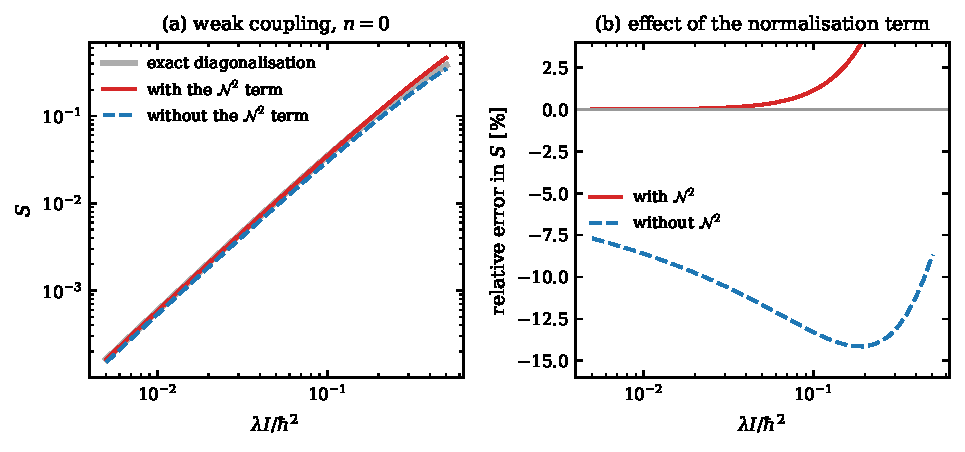
\includegraphics[width=\linewidth]{fig1_weak.pdf}
\caption{(a) Entanglement entropy at weak coupling for $n=0$ ($m_{1}=m_{2}=4$):
exact diagonalisation (grey), Eq.~\eqref{eq:Sweak} (red), and the same
expression with the normalisation term of \eqref{eq:rho} removed (blue dashed).
(b) Relative error of the two truncations. With the term the error is
$0.05\%$ at $\lambda I/\hbar^{2}=0.02$ and $1\%$ at $0.1$, decreasing as
$\lambda^{2}$; without it the deficit is $10$--$14\%$ and does not vanish as
$\lambda\to0$.}
\label{fig:weak}
\end{figure}

%=============================================================================
\section{Beyond perturbation theory: the Mathieu equation}
\label{sec:pendulum}
%=============================================================================

\subsection{The sector Hamiltonian}

Inside sector $M$ label the states by $m\equiv m_{1}$, so $m_{2}=M-m$. Completing
the square,
\begin{equation}
m^{2}+(M-m)^{2}=2m^{2}-2Mm+M^{2}=2\left(m-\tfrac{M}{2}\right)^{2}+\tfrac{M^{2}}{2},
\end{equation}
so by \eqref{eq:E0}
\begin{equation}
E^{(0)}=\frac{\hbar^{2}M^{2}}{4I}+\frac{\hbar^{2}}{I}\,k^{2},
\qquad k\equiv m-\frac{M}{2}=\frac{n}{2}.
\end{equation}
The coupling connects $m$ with $m\pm1$, i.e.\ $k$ with $k\pm1$, with strength
$\lambda/2$. Hence
\begin{equation}
H\big|_{\mathcal{H}_{M}}=\frac{\hbar^{2}M^{2}}{4I}+h,\qquad
h_{kk'}=\frac{\hbar^{2}}{I}k^{2}\,\delta_{kk'}
+\frac{\lambda}{2}\left(\delta_{k',k+1}+\delta_{k',k-1}\right),
\label{eq:hsector}
\end{equation}
a real symmetric tridiagonal matrix. The label $k$ runs over $\mathbb{Z}$ if $M$
is even and over $\mathbb{Z}+\tfrac12$ if $M$ is odd. Consequently every
even-$M$ sector is identical to $M=0$ and every odd-$M$ sector to $M=1$, up to
the constant $\hbar^{2}M^{2}/4I$; we verify this numerically in
Table~\ref{tab:checks}.

\subsection{Identification with the pendulum}

In sector $M$ the wave function factorises in the variables \eqref{eq:cmrel}:
\begin{equation}
e^{im_{1}\theta_{1}+im_{2}\theta_{2}}
=e^{i(m_{1}+m_{2})\Theta}\,e^{i(m_{1}-m_{2})\varphi/2}
=e^{iM\Theta}\,e^{ik\varphi},
\end{equation}
so $\Psi(\theta_{1},\theta_{2})=e^{iM\Theta}u(\varphi)/\sqrt{2\pi}$ with
$u(\varphi)=\sum_{k}c_{k}\,e^{ik\varphi}/\sqrt{2\pi}$. For even $M$, $k$ is an
integer and $u(\varphi+2\pi)=u(\varphi)$; for odd $M$, $k$ is a half-integer and
$u(\varphi+2\pi)=-u(\varphi)$. Now consider
\begin{equation}
h=-\frac{\hbar^{2}}{I}\frac{\dd^{2}}{\dd\varphi^{2}}+\lambda\cos\varphi .
\label{eq:mathieuop}
\end{equation}
Acting on $\chi_{k}(\varphi)=e^{ik\varphi}/\sqrt{2\pi}$, the derivative term
gives $(\hbar^{2}/I)k^{2}\chi_{k}$ and
$\lambda\cos\varphi\,\chi_{k}=\tfrac{\lambda}{2}(\chi_{k+1}+\chi_{k-1})$, so the
matrix of \eqref{eq:mathieuop} in the basis $\chi_{k}$ is exactly
\eqref{eq:hsector}. This is the relative Hamiltonian $H_{\rm rel}$ of
\eqref{eq:Hcm}, quantised with $p=-i\hbar\,\partial_{\varphi}$: \emph{each sector
of the two-rotor problem is exactly the quantum pendulum}, with periodic
boundary conditions for even $M$ and antiperiodic ones for odd $M$.

\subsection{Reduction to the standard Mathieu equation}

The eigenvalue equation $h u=\Erel u$ reads
$-(\hbar^{2}/I)u''+\lambda\cos\varphi\,u=\Erel u$. Substituting $\varphi=2z$,
so that $\dd^{2}/\dd\varphi^{2}=\tfrac14\dd^{2}/\dd z^{2}$, and multiplying by
$-4I/\hbar^{2}$,
\begin{equation}
\frac{\dd^{2}u}{\dd z^{2}}+\left(a-2q\cos2z\right)u=0,\qquad
\boxed{\;a=\frac{4I\Erel}{\hbar^{2}},\qquad q=\frac{2\lambda I}{\hbar^{2}}
=4\alpha\;}
\label{eq:mathieu}
\end{equation}
the Mathieu equation in standard form~\cite{DLMF28,AbramowitzStegun}. A
$2\pi$-periodic $u(\varphi)$ is $\pi$-periodic in $z$; the corresponding
solutions are $\mathrm{ce}_{2r}(z,q)$ (even) and $\mathrm{se}_{2r+2}(z,q)$
(odd), with characteristic values $a_{2r}(q)$ and $b_{2r+2}(q)$. An
antiperiodic $u(\varphi)$ is $\pi$-antiperiodic in $z$; the solutions are
$\mathrm{ce}_{2r+1}$ and $\mathrm{se}_{2r+1}$, with $a_{2r+1}(q)$, $b_{2r+1}(q)$.
Therefore
\begin{equation}
E=\frac{\hbar^{2}M^{2}}{4I}+\frac{\hbar^{2}}{4I}\times
\begin{cases}a_{0}<b_{2}<a_{2}<b_{4}<\dots, & M\ \text{even},\\[2pt]
b_{1}<a_{1}<b_{3}<a_{3}<\dots, & M\ \text{odd},\end{cases}
\label{eq:Emathieu}
\end{equation}
which we have checked to all printed digits against exact diagonalisation
(Table~\ref{tab:checks}). The orderings follow from the interlacing
$a_{0}<b_{1}<a_{1}<b_{2}<a_{2}<\dots$ valid for $q>0$; for odd $M$ the lowest
level is $b_{1}$, whose eigenfunction $\mathrm{se}_{1}\sim\sin z$ is largest at the
potential minimum $z=\pi/2$. The separatrix $\Erel=\lambda$ is at $a=2q$. Parity
$z\to-z$ is the exchange $P$ of Sec.~\ref{sec:exchange}: $\mathrm{ce}$ and
$\mathrm{se}$ are its even and odd eigenfunctions.

The number of librating levels follows from the Bohr--Sommerfeld rule: the
area enclosed by the separatrix
$p=\pm\sqrt{I\lambda(1-\cos\varphi)}=\pm\sqrt{2I\lambda}\,|\sin(\varphi/2)|$ is
$\oint p\,\dd\varphi=2\sqrt{2I\lambda}\int_{0}^{2\pi}\sin(\varphi/2)\dd\varphi
=8\sqrt{2I\lambda}$, and dividing by $2\pi\hbar$,
\begin{equation}
N_{\rm lib}\simeq\frac{8\sqrt{2I\lambda}}{2\pi\hbar}=\frac{4}{\pi}\sqrt{q}.
\end{equation}
For $\lambda I/\hbar^{2}=50,200,800,3200$ this gives $12.7,25.5,50.9,101.9$,
against $13,25,51,102$ counted.

\subsection{The entanglement entropy is a Shannon entropy}

For an eigenstate $\Psi=e^{iM\Theta}u(\varphi)/\sqrt{2\pi}$ with
$u=\sum_{k}c_{k}\chi_{k}$, the state is
\begin{equation}
\ket\Psi=\sum_{k}c_{k}\,\ket{m_{1}=\tfrac{M}{2}+k,\;m_{2}=\tfrac{M}{2}-k}.
\end{equation}
Each value of $m_{1}$ appears with a single $m_{2}$, so by \eqref{eq:ptrace}
\begin{equation}
\rho_{1}=\sum_{k}|c_{k}|^{2}\,\ketbra{\tfrac{M}{2}+k}{\tfrac{M}{2}+k},
\qquad
\boxed{\;S=-\sum_{k}|c_{k}|^{2}\ln|c_{k}|^{2}\;}
\label{eq:Smathieu}
\end{equation}
exactly, to all orders in $\lambda$. \emph{The entanglement entropy of the two
rotors is the Shannon entropy of the Fourier coefficients of the Mathieu
function.} The Schmidt basis is fixed by angular-momentum conservation, and the
entropy depends on $M$ only through its parity (and through $\Erel$). The
perturbative result \eqref{eq:rho1} is the small-$q$ expansion of
\eqref{eq:Smathieu}.

\subsection{Parity sectors in the plane-wave basis}

Above the separatrix the levels of \eqref{eq:mathieuop} form exponentially close
doublets (counter-rotating states), so a dense eigensolver applied to
\eqref{eq:hsector} returns arbitrary mixtures of the two members. We diagonalise
in the eigenspaces of $P:k\to-k$ separately. For even $M$ the even sector has
basis $\{\chi_{0},(\chi_{k}+\chi_{-k})/\sqrt2\}_{k\ge1}$, in which
\begin{equation}
\bra{\chi_{0}}h\,\tfrac{1}{\sqrt2}(\chi_{1}+\chi_{-1})
=\tfrac{1}{\sqrt2}\left(\tfrac{\lambda}{2}+\tfrac{\lambda}{2}\right)
=\tfrac{\lambda}{\sqrt2},
\end{equation}
while all other off-diagonal elements are $\lambda/2$; the odd sector has basis
$\{(\chi_{k}-\chi_{-k})/\sqrt2\}_{k\ge1}$ with off-diagonal elements $\lambda/2$.
For odd $M$ the even and odd combinations of $\chi_{\pm1/2}$ acquire diagonal
elements $\hbar^{2}/4I\pm\lambda/2$: the coupling $\chi_{1/2}\leftrightarrow
\chi_{-1/2}$ splits the $n=\pm1$ pair at first order, which is the resonance of
Sec.~\ref{sec:pt} seen from the exact side.

%=============================================================================
\section{Classical entanglement entropy}
\label{sec:classical}
%=============================================================================

\subsection{The microcanonical distribution}

The classical Hamiltonian is \eqref{eq:H} with real $p_{i}$. It is integrable,
with two independent integrals in involution, $E$ and $J$. Following~\cite{DKS},
the classical counterpart of an eigenstate with definite energy and total
angular momentum is the microcanonical distribution on the corresponding level
set,
\begin{equation}
W(\theta_{1},p_{1};\theta_{2},p_{2})=\mathcal{C}\;
\delta\!\left(E-H\right)\,\delta\!\left(J-p_{1}-p_{2}\right),
\label{eq:Wjoint}
\end{equation}
normalised by $\int\dd\theta_{1}\dd p_{1}\dd\theta_{2}\dd p_{2}\,W=1$. By
Liouville's theorem this measure is invariant under the flow; on each invariant
torus it is uniform in the angle variables, which is the same as the time
average along a generic orbit. One point deserves attention. For
$\Erel>\lambda$ the level set consists of \emph{two} tori, $p>0$ and $p<0$
(the two senses of relative rotation), and \eqref{eq:Wjoint} weights them
equally; for $|\Erel|<\lambda$ there is one torus. This matches the quantum
side, where the exact eigenstates are parity eigenstates, symmetric under
$p\to-p$.

\subsection{Integrating out the second rotor}

The reduced distribution of rotor 1 is
$W(\theta_{1},p_{1})=\int\dd\theta_{2}\,\dd p_{2}\,W$. The second delta
function fixes $p_{2}=J-p_{1}$:
\begin{equation}
W(\theta_{1},p_{1})=\mathcal{C}\int_{0}^{2\pi}\dd\theta_{2}\;
\delta\!\left(E-K(p_{1})-\lambda\cos(\theta_{1}-\theta_{2})\right),\qquad
K(p_{1})=\frac{p_{1}^{2}+(J-p_{1})^{2}}{2I}.
\end{equation}
With $p_{1}=J/2+p$ the identity $p_{1}^{2}+(J-p_{1})^{2}=J^{2}/2+2p^{2}$ gives
$E-K=\Erel-p^{2}/I$. Changing variable to $\varphi=\theta_{1}-\theta_{2}$
($|\dd\varphi|=|\dd\theta_{2}|$) and using periodicity to shift the interval of
integration to a full period,
\begin{equation}
W(\theta_{1},p_{1})=\mathcal{C}\int_{0}^{2\pi}\dd\varphi\;
\delta\!\left(g(\varphi)\right),\qquad
g(\varphi)=\Erel-\frac{p^{2}}{I}-\lambda\cos\varphi .
\end{equation}
For a function with simple zeros $\varphi_{j}$,
$\delta(g(\varphi))=\sum_{j}\delta(\varphi-\varphi_{j})/|g'(\varphi_{j})|$. Here
$g'(\varphi)=\lambda\sin\varphi$, and $g(\varphi_{j})=0$ means
$\cos\varphi_{j}=\xi\equiv(\Erel-p^{2}/I)/\lambda$. For $|\xi|<1$ there are two
zeros in $[0,2\pi)$, $\varphi=\pm\arccos\xi$, each with
$|g'|=\lambda\sqrt{1-\xi^{2}}=\sqrt{\lambda^{2}-(\Erel-p^{2}/I)^{2}}$; for
$|\xi|>1$ there are none. Hence
\begin{equation}
\boxed{\;
W(\theta_{1},p_{1})=\frac{2\mathcal{C}}
{\sqrt{\lambda^{2}-\left(\Erel-p^{2}/I\right)^{2}}}\;
\Theta\!\left(\lambda-\left|\Erel-p^{2}/I\right|\right),\qquad p=p_{1}-\frac{J}{2}\;}
\label{eq:Wclass}
\end{equation}
independent of $\theta_{1}$, as it must be: no absolute angle is distinguished.
The classical correlation is carried entirely by the momentum. Rotor 1 is
constrained by the requirement that the interaction energy $\Erel-p^{2}/I$ lie
in the range $[-\lambda,\lambda]$ accessible to $\lambda\cos\varphi$, and this
constraint, inherited from the unobserved rotor, spreads $p_{1}$ over a band.

\subsection{The support and its cusp at the separatrix}

The band $|\Erel-p^{2}/I|\le\lambda$ is
\begin{equation}
\begin{aligned}
&|p|\le\sqrt{I(\Erel+\lambda)}, &&-\lambda<\Erel<\lambda\quad\text{(libration)},\\
&\sqrt{I(\Erel-\lambda)}\le|p|\le\sqrt{I(\Erel+\lambda)}, &&\Erel>\lambda
\quad\text{(rotation)},
\end{aligned}
\end{equation}
with total length
\begin{equation}
L(\Erel)=\begin{cases}2\sqrt{I(\Erel+\lambda)}, & \Erel<\lambda,\\[2pt]
2\left[\sqrt{I(\Erel+\lambda)}-\sqrt{I(\Erel-\lambda)}\right], & \Erel>\lambda .
\end{cases}
\label{eq:support}
\end{equation}
$L$ increases through the libration regime, reaches its maximum
$2\sqrt{2I\lambda}$ at the separatrix, and decreases above it, with
$\dd L/\dd\Erel\to-\infty$ as $\Erel\to\lambda^{+}$ because of the
$-\sqrt{\Erel-\lambda}$ term. The support therefore has a cusp maximum at the
separatrix. Since the entropy of a distribution on a set of length $L$ is at
most $\ln(L/\hbar)$, this is the origin of the entropy maximum found in
Sec.~\ref{sec:compare}.

\subsection{Normalisation and the classical period}

Integrating \eqref{eq:Wclass} over $\theta_{1}$ gives the momentum density
$w(p_{1})=2\pi W$. Its normalisation requires the band integral
\begin{equation}
B(\Erel)\equiv\int_{\rm band,\;p>0}
\frac{\dd p}{\sqrt{\lambda^{2}-(\Erel-p^{2}/I)^{2}}} .
\end{equation}
Substitute $\Erel-p^{2}/I=\lambda\cos u$: then $p=\sqrt{I(\Erel-\lambda\cos u)}$,
$\dd p=I\lambda\sin u\,\dd u/(2p)$ and
$\sqrt{\lambda^{2}-\lambda^{2}\cos^{2}u}=\lambda\sin u$, so
\begin{equation}
B=\frac{I}{2}\int\frac{\dd u}{p(u)}
=\frac{\sqrt{I}}{2}\int\frac{\dd u}{\sqrt{\Erel-\lambda\cos u}} .
\end{equation}
\emph{Rotation} ($\Erel>\lambda$): $u\in[0,\pi]$. With $u=\pi-2t$,
$\cos u=-\cos2t=-1+2\sin^{2}t$ and
$\Erel-\lambda\cos u=(\Erel+\lambda)(1-k^{2}\sin^{2}t)$ with
$k^{2}=2\lambda/(\Erel+\lambda)<1$, whence
\begin{equation}
B=\frac{\sqrt I}{2}\cdot\frac{2}{\sqrt{\Erel+\lambda}}\int_{0}^{\pi/2}
\frac{\dd t}{\sqrt{1-k^{2}\sin^{2}t}}
=\sqrt{\frac{I}{\Erel+\lambda}}\;\mathsf{K}(k),\qquad
k^{2}=\frac{2\lambda}{\Erel+\lambda}.
\label{eq:Brot}
\end{equation}
\emph{Libration} ($|\Erel|<\lambda$): $p^{2}\ge0$ restricts $u$ to
$[u_{0},\pi]$ with $\cos u_{0}=\Erel/\lambda$. With $v=\pi-u$ and
$\sin(v/2)=\kappa\sin t$, $\kappa^{2}=(\Erel+\lambda)/2\lambda<1$, one finds
$\Erel+\lambda\cos v=(\Erel+\lambda)\cos^{2}t$ and
$\dd v=2\kappa\cos t\,\dd t/\sqrt{1-\kappa^{2}\sin^{2}t}$, so that
\begin{equation}
B=\frac{\sqrt I}{2}\cdot\frac{2\kappa}{\sqrt{\Erel+\lambda}}\int_{0}^{\pi/2}
\frac{\dd t}{\sqrt{1-\kappa^{2}\sin^{2}t}}
=\sqrt{\frac{I}{2\lambda}}\;\mathsf{K}(\kappa),\qquad
\kappa^{2}=\frac{\Erel+\lambda}{2\lambda}.
\label{eq:Blib}
\end{equation}
Here $\mathsf{K}$ is the complete elliptic integral of the first kind. Both forms
agree with direct quadrature to eight digits (\ref{app:num}). In either regime
the momentum density has total weight $2B$ over all $p$ (two bands, or one band
symmetric in $p$), so
\begin{equation}
\mathcal{C}=\frac{1}{8\pi B},\qquad
w(p_{1})=\frac{1}{2B}\,\frac{1}{\sqrt{\lambda^{2}-(\Erel-p^{2}/I)^{2}}}.
\end{equation}
The band integral is, up to a constant, the classical period: with
$\dot\varphi=\partial H_{\rm rel}/\partial p=2p/I$,
$\dd t=I\dd\varphi/2p$, and the same substitution shows that the period of
rotation is $T=2B$. At the separatrix $k,\kappa\to1$ and
$\mathsf{K}\simeq\ln\big(4/\sqrt{1-k^{2}}\big)$ diverges logarithmically: the
orbit lingers near the unstable point $\varphi=0$, where $p\to0$.

\subsection{Boltzmann entropy and the elementary cell}
\label{sec:cell}

The Boltzmann entropy of the reduced distribution is
\begin{equation}
\Scl=-\int\dd\theta_{1}\,\dd p_{1}\;W\ln\left(W\Delta\right),
\label{eq:Sclass}
\end{equation}
with $\Delta$ an elementary area making $W\Delta$ dimensionless. On a compact
configuration space $\Delta$ is not free. Single-valuedness quantises
$p_{1}=\hbar m_{1}$, so each quantum state occupies the strip
$\Delta\theta_{1}\times\Delta p_{1}=2\pi\times\hbar=h$, and $\Delta=h$. Because
$W=w(p_{1})/2\pi$ is independent of $\theta_{1}$, \eqref{eq:Sclass} reduces to
\begin{equation}
\Scl=-\int\dd p_{1}\;w\ln\left(w\hbar\right),
\label{eq:Sdiff}
\end{equation}
a differential entropy in units of $\hbar$. The object with the same status as
the quantum entropy \eqref{eq:Smathieu} --- a Shannon entropy over the integers
--- is obtained by integrating $w$ over the unit cells:
\begin{equation}
w_{m}=\int_{\hbar(m-1/2)}^{\hbar(m+1/2)}w(p_{1})\,\dd p_{1},\qquad
\sum_{m}w_{m}=1,\qquad
\Scl^{\rm bin}=-\sum_{m}w_{m}\ln w_{m}.
\label{eq:Sbin}
\end{equation}
The comparison between \eqref{eq:Sbin} and \eqref{eq:Smathieu} contains no
adjustable constant. The two classical expressions are related as follows. On
cell $m$ let $\varrho(p)=w(p)/w_{m}$, a normalised density on an interval of
length $\hbar$. Then
\begin{equation}
\Scl=-\sum_{m}w_{m}\int_{\rm cell}\varrho\ln\left(w_{m}\varrho\hbar\right)\dd p
=\Scl^{\rm bin}-\sum_{m}w_{m}\,D_{\rm KL}\!\left(\varrho\,\Vert\,
\hbar^{-1}\right),
\end{equation}
where $D_{\rm KL}(\varrho\Vert\hbar^{-1})=\int\varrho\ln(\varrho\hbar)\,\dd p
\ge0$ is the relative entropy of $\varrho$ with respect to the uniform density on
the cell. Hence $\Scl^{\rm bin}\ge\Scl$, with equality when $w$ is constant on
each cell: coarse-graining raises the entropy. The difference comes mainly from
the cells containing the inverse-square-root singularities at the band edges,
whose weight decreases as $(\text{band width in cells})^{-1/2}$; for the arcsine
law of Sec.~\ref{sec:rotation} we find $\Scl^{\rm bin}-\Scl=0.20,0.064,0.020$
for $\gamma=10,100,1000$, decreasing as $\gamma^{-1/2}$.

%=============================================================================
\section{Deep rotation: an exactly solvable limit and the constant $1-\ln2$}
\label{sec:rotation}
%=============================================================================

\subsection{Reduction to a Wannier--Stark ladder}

Consider a level with large relative angular momentum, $k_{0}=n/2\gg1$, and
write $k=k_{0}+j$. Then
\begin{equation}
\frac{\hbar^{2}}{I}k^{2}=\frac{\hbar^{2}}{I}k_{0}^{2}+F\,j+\frac{\hbar^{2}}{I}j^{2},
\qquad F\equiv\frac{2\hbar^{2}k_{0}}{I}=\frac{\hbar^{2}n}{I}.
\end{equation}
Over the range of $j$ that will turn out to matter, $|j|\lesssim\gamma$ with
$\gamma$ defined below, the quadratic term is smaller than the linear one by
$|j|/n\le\gamma/n$. Dropping it, \eqref{eq:hsector} becomes, up to the constant
$\hbar^{2}k_{0}^{2}/I$,
\begin{equation}
h_{\rm WS}\,c_{j}=F\,j\,c_{j}+\frac{\lambda}{2}\left(c_{j+1}+c_{j-1}\right),
\label{eq:WS}
\end{equation}
a particle hopping on a lattice in a uniform field: the Wannier--Stark problem.
Its eigenvectors follow from the Bessel recurrence
$J_{\nu-1}(x)+J_{\nu+1}(x)=(2\nu/x)J_{\nu}(x)$. Try $c_{j}=J_{j-s}(x)$ with
$s\in\mathbb{Z}$:
\begin{equation}
\frac{\lambda}{2}\left(c_{j+1}+c_{j-1}\right)
=\frac{\lambda}{2}\cdot\frac{2(j-s)}{x}J_{j-s}(x)=\frac{\lambda(j-s)}{x}c_{j},
\end{equation}
so $h_{\rm WS}c_{j}=\left[Fj+\lambda(j-s)/x\right]c_{j}$. This is independent of
$j$, as an eigenvalue must be, if and only if $x=-\lambda/F$; the eigenvalue is
then $Fs$. Using $J_{\nu}(-x)=(-1)^{\nu}J_{\nu}(x)$, the eigenvector centred on
$s$ has
\begin{equation}
|c_{j}|^{2}=J_{j-s}^{2}(\gamma),\qquad
\boxed{\;\gamma\equiv\frac{\lambda}{F}=\frac{\lambda I}{\hbar^{2}n}
=\frac{2\alpha}{n}\;}
\label{eq:bessel}
\end{equation}
Normalisation is the Neumann identity $\sum_{j}J_{j}^{2}(\gamma)=1$. The
Wannier--Stark levels $Fs$ are equally spaced and non-degenerate, and the
eigenvectors are translates of one another, so all have the same entropy.

\emph{Validity.} The neglected term is small when $\gamma\ll n$, i.e.
$\lambda I/\hbar^{2}\ll n^{2}$; with $\Erel\simeq\hbar^{2}n^{2}/4I$ this is
$\gamma/n=\lambda/4\Erel\ll1$, deep in the rotation regime. Exact
diagonalisation confirms \eqref{eq:bessel} pointwise to $3\times10^{-3}$ at
$\gamma=2,5$ ($\gamma/n=0.01$), and the entropy to four or five digits for
$n=100$--$400$ (Fig.~\ref{fig:rotation}a).

\subsection{The entanglement entropy as a function of one variable}

From \eqref{eq:Smathieu} and \eqref{eq:bessel}, the branch entropy in deep
rotation is a universal function of $\gamma$ alone:
\begin{equation}
\boxed{\;S_{\rm branch}(\gamma)=-\sum_{j\in\mathbb{Z}}J_{j}^{2}(\gamma)\ln
J_{j}^{2}(\gamma)\;}
\label{eq:SB}
\end{equation}
(for the exact parity eigenstate add $\ln2$, Sec.~\ref{sec:ln2}). Its two limits
are the perturbative and the classical regimes.

\emph{Small $\gamma$.} From $J_{0}(\gamma)=1-\gamma^{2}/4+\dots$ and
$J_{\pm1}(\gamma)=\pm\gamma/2+\dots$, the weights are
$1-\gamma^{2}/2$ and $\gamma^{2}/4$ (twice), so
\begin{equation}
S_{\rm branch}\simeq2\cdot\frac{\gamma^{2}}{4}\ln\frac{4}{\gamma^{2}}
+\frac{\gamma^{2}}{2}=\gamma^{2}\left[\ln\frac{2}{\gamma}+\frac12\right].
\end{equation}
Since $\gamma^{2}/4=\alpha^{2}/n^{2}\simeq\varepsilon_{\pm}$, this is exactly the
large-$n$ perturbative result \eqref{eq:Sasym}, including the factor $2$ in the
logarithm and the normalisation term $\tfrac12$.

\emph{Large $\gamma$.} Here the weights become many and the classical
description applies; we treat this next.

\subsection{The classical counterpart: the arcsine law}

In the same limit the classical density \eqref{eq:Wclass} simplifies. Near
$p_{0}=\sqrt{I\Erel}$, linearise $p^{2}/I\simeq p_{0}^{2}/I+2p_{0}(p-p_{0})/I$, so
that $\Erel-p^{2}/I\simeq-2p_{0}(p-p_{0})/I$ and
\begin{equation}
w\propto\frac{1}{\sqrt{\lambda^{2}-4p_{0}^{2}(p-p_{0})^{2}/I^{2}}}
\propto\frac{1}{\sqrt{a^{2}-(p-p_{0})^{2}}},\qquad a=\frac{I\lambda}{2p_{0}}.
\end{equation}
In units of $\hbar$, with $p_{0}=\hbar n/2$, the half-width is
$a/\hbar=\lambda I/\hbar^{2}n=\gamma$. The classical weights are the arcsine law
on $|j|<\gamma$,
\begin{equation}
w(j)=\frac{1}{\pi\sqrt{\gamma^{2}-j^{2}}},
\label{eq:arcsine}
\end{equation}
and its differential entropy is (\ref{app:integrals})
\begin{equation}
\Scl=-\int_{-\gamma}^{\gamma}w\ln w\,\dd j=\ln\frac{\pi\gamma}{2}.
\label{eq:Sarcsine}
\end{equation}
For the parity-symmetric distribution, which consists of two such bands of
equal weight at $\pm p_{0}$, one adds $\ln2$. Using $\hbar n=2\sqrt{I\Erel}$,
$\gamma=\lambda I/\hbar^{2}n=(\lambda/2\hbar)\sqrt{I/\Erel}$, so
\begin{equation}
\Scl^{\,\rm branch}=\ln\frac{\pi\gamma}{2},\qquad
\Scl^{\,\rm two\ bands}=\ln(\pi\gamma)
=\ln\left[\frac{\pi\lambda}{2\hbar}\sqrt{\frac{I}{\Erel}}\,\right].
\label{eq:Sclrot}
\end{equation}
This is the rotor counterpart of the DKS result \eqref{eq:DKSresult}: the
entropy grows logarithmically with the coupling and decreases logarithmically
with the energy of the relative motion, and it becomes negative --- the
classical description fails --- when $\gamma<2/\pi$, i.e.\ when the band covers
less than about one cell.

\subsection{Interference fringes in the quantum weights}

The quantum weights are not the arcsine law: they oscillate about it. The
Debye expansion of the Bessel function~\cite{DLMF10}, written with
$j=\gamma\cos\beta$, $0<\beta<\pi$, reads
\begin{equation}
J_{j}(\gamma)\simeq\sqrt{\frac{2}{\pi\gamma\sin\beta}}\,
\cos\left(\gamma\sin\beta-j\beta-\frac{\pi}{4}\right).
\end{equation}
Squaring, with $\gamma\sin\beta=\sqrt{\gamma^{2}-j^{2}}$ and
$\cos^{2}x=\tfrac12(1+\cos2x)$,
\begin{equation}
J_{j}^{2}(\gamma)\simeq w(j)\left[1+\cos\Phi_{j}\right],\qquad
\Phi_{j}=2\sqrt{\gamma^{2}-j^{2}}-2j\arccos\frac{j}{\gamma}-\frac{\pi}{2},
\label{eq:fringes}
\end{equation}
with $w(j)$ the arcsine law \eqref{eq:arcsine}. The quantum weights are the
classical ones modulated by fringes of \emph{full} contrast. Their origin is the
interference of the two classical relative angles $\varphi=\pm\arccos\xi$ that
correspond to the same momentum. The local fringe wavenumber is
\begin{equation}
\frac{\dd\Phi_{j}}{\dd j}=-\frac{2j}{\sqrt{\gamma^{2}-j^{2}}}
-2\arccos\frac{j}{\gamma}+\frac{2j}{\sqrt{\gamma^{2}-j^{2}}}=-2\beta,
\end{equation}
which ranges over $(-2\pi,0)$ across the band.

The same structure holds at any energy. In the $k$ representation the
eigenvalue equation $\frac{\hbar^{2}}{I}k^{2}c_{k}+\frac{\lambda}{2}(c_{k+1}+
c_{k-1})=\Erel c_{k}$ is a difference equation, and the WKB ansatz
$c_{k}=A_{k}e^{i\chi_{k}}$ with slowly varying $A_{k}$ and local wavenumber
$\phi_{k}=\chi_{k+1}-\chi_{k}$ gives at leading order
$\Erel-\hbar^{2}k^{2}/I=\lambda\cos\phi_{k}$, which is the classical relation
between the relative momentum $\hbar k$ and the relative angle. The two roots
$\pm\phi_{k}$ give two solutions. The Casoratian
$\mathcal{W}_{k}=\tfrac{\lambda}{2}(c_{k}\bar c_{k+1}-c_{k+1}\bar c_{k})$ of
any two solutions is independent of $k$, which for a single WKB wave gives
$|A_{k}|^{2}\lambda\sin\phi_{k}={\rm const}$, i.e.\
$|A_{k}|^{2}\propto1/\sqrt{\lambda^{2}-(\Erel-\hbar^{2}k^{2}/I)^{2}}$: the
classical density \eqref{eq:Wclass}. A real eigenvector is a superposition of
the two waves with equal amplitude, so in general
\begin{equation}
|c_{k}|^{2}\simeq w_{k}\left(1+\cos\Phi_{k}\right),\qquad
\Phi_{k+1}-\Phi_{k}=2\phi_{k}.
\label{eq:fringesgen}
\end{equation}
The classical distribution is the fringe average of the quantum one.

\subsection{The entropy deficit}

Insert $p_{k}=w_{k}(1+\cos\Phi_{k})$ into $S_{q}=-\sum p_{k}\ln p_{k}$:
\begin{align}
S_{q}&=-\sum_{k}w_{k}(1+\cos\Phi_{k})\left[\ln w_{k}+\ln(1+\cos\Phi_{k})\right]
\nonumber\\
&=\Scl^{\rm bin}-\sum_{k}w_{k}\cos\Phi_{k}\ln w_{k}
-\sum_{k}w_{k}(1+\cos\Phi_{k})\ln(1+\cos\Phi_{k}).
\end{align}
In the second term $\cos\Phi_{k}$ oscillates on the scale of a few cells while
$w_{k}\ln w_{k}$ varies on the scale of the band, so the sum vanishes as the
band widens (the discrete analogue of the Riemann--Lebesgue lemma). In the
third, the phases $\Phi_{k}\bmod2\pi$ are equidistributed wherever the
increment $2\phi_{k}$ is not close to a multiple of $2\pi$, and the sum becomes
a phase average:
\begin{equation}
\Scl-S_{q}\;\longrightarrow\;\frac{1}{2\pi}\int_{0}^{2\pi}
(1+\cos\Phi)\ln(1+\cos\Phi)\,\dd\Phi=1-\ln2 .
\label{eq:deficit}
\end{equation}
The integral is evaluated in \ref{app:integrals}. Thus
\begin{equation}
\boxed{\;S_{q}=\Scl-\left(1-\ln2\right)+o(1)\;}\qquad
1-\ln2=0.30685\ldots
\label{eq:main}
\end{equation}
in the semiclassical limit. The limiting deficit is universal: it does not
depend on $\lambda$, $n$, $M$, or the energy, only on the full contrast of the
two-branch interference.

\emph{Rate of approach.} Equidistribution fails near the band edges, where
$\phi_{k}\to0$ or $\pi$ and the fringes become stationary (the caustics of the
momentum-space WKB, where it is replaced by an Airy function). Near the edge
$j=\gamma-\delta$ one has $\beta\simeq\sqrt{2\delta/\gamma}$, so the phase
accumulated over the last $\delta$ cells is
$\int2\beta\,\dd j\simeq\tfrac{4\sqrt2}{3}\delta^{3/2}/\sqrt\gamma$. This reaches
$2\pi$ at $\delta\sim\gamma^{1/3}$, and the arcsine weight within that distance
of the edge is $\pi^{-1}\arccos(1-\delta/\gamma)\simeq\pi^{-1}\sqrt{2\delta/\gamma}
\sim\gamma^{-1/3}$. Hence
\begin{equation}
\Scl-S_{q}=1-\ln2-O\!\left(\gamma^{-1/3}\right).
\end{equation}

\subsection{Numerical confirmation}

Because \eqref{eq:bessel} is explicit, \eqref{eq:main} can be tested to very
large $\gamma$ by summing $J_{j}^{2}$ directly. Figure~\ref{fig:rotation}(b)
shows $\Scl^{\rm bin}-S_{q}$ for $\gamma=10$ to $10^{6}$. It rises
monotonically, $0.233$ at $\gamma=10^{3}$, $0.270$ at $10^{4}$, $0.288$ at
$10^{5}$ and $0.298$ at $10^{6}$, and the distance to $1-\ln2$ halves per decade,
consistent with $\gamma^{-1/3}$ (a factor $2.15$ per decade).

\begin{figure}[t]
\centering
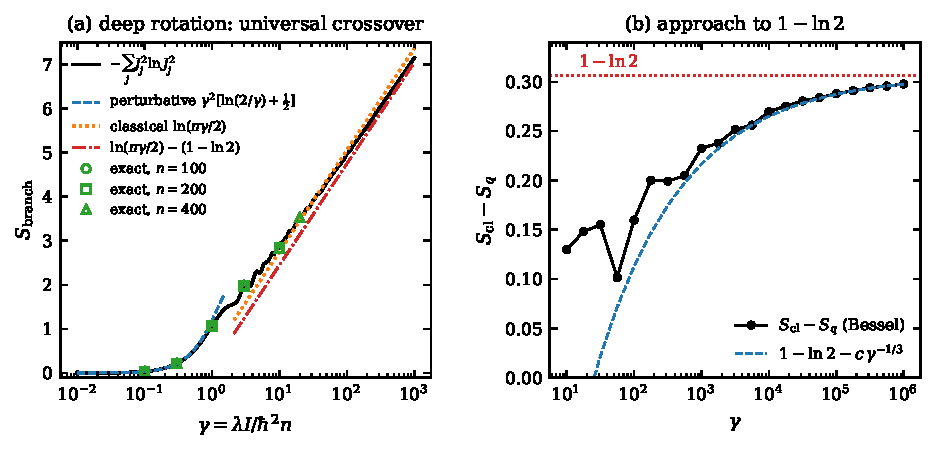
\includegraphics[width=\linewidth]{fig2_rotation.pdf}
\caption{Deep rotation. (a) The branch entropy as a universal function of
$\gamma=\lambda I/\hbar^{2}n$: the Bessel result \eqref{eq:SB} (black), its
perturbative limit (blue dashed), the classical arcsine entropy (orange dotted)
and the classical entropy minus $1-\ln2$ (red dash-dotted). Open symbols: exact
diagonalisation at $n=100,200,400$. (b) The deficit $\Scl^{\rm bin}-S_{q}$ from
the Bessel weights, approaching $1-\ln2$ as $\gamma^{-1/3}$.}
\label{fig:rotation}
\end{figure}

\subsection{Interpretation}

The oscillator pair of~\cite{DKS} and the rotor pair differ in one structural
respect. In the oscillator case no conservation law singles out a Schmidt
basis; the reduced density matrix found in~\cite{DKS} is doubly degenerate,
with eigenvalues following the smooth arcsine law and with the
two-branch interference absorbed into the eigenvectors. For the rotors,
conservation of $J$ forces the Schmidt basis to be the angular-momentum basis
(Sec.~\ref{sec:pendulum}), so the interference cannot be absorbed into the
eigenvectors and appears in the eigenvalues themselves, as the fringes
\eqref{eq:fringesgen}. The leading logarithms of the quantum and classical
entropies agree, as in the oscillator case; the constant term does not, and the
difference is $1-\ln2$. Equivalently, the classical formula \eqref{eq:Sdiff}
reproduces the quantum entropy if the cell is taken to be $\Delta=eh/2$ rather
than $h$, since $\ln(e/2)=1-\ln2$.

%=============================================================================
\section{Generic energies and the separatrix}
\label{sec:compare}
%=============================================================================

Away from deep rotation we compare \eqref{eq:Smathieu}, computed by exact
diagonalisation in the parity sectors, with \eqref{eq:Sbin}, computed by
adaptive quadrature of \eqref{eq:Wclass} over each cell.
Figure~\ref{fig:separatrix} shows both for $\lambda I/\hbar^{2}=50,200,800$ as a
function of $\Erel/\lambda$.

\begin{figure}[t]
\centering
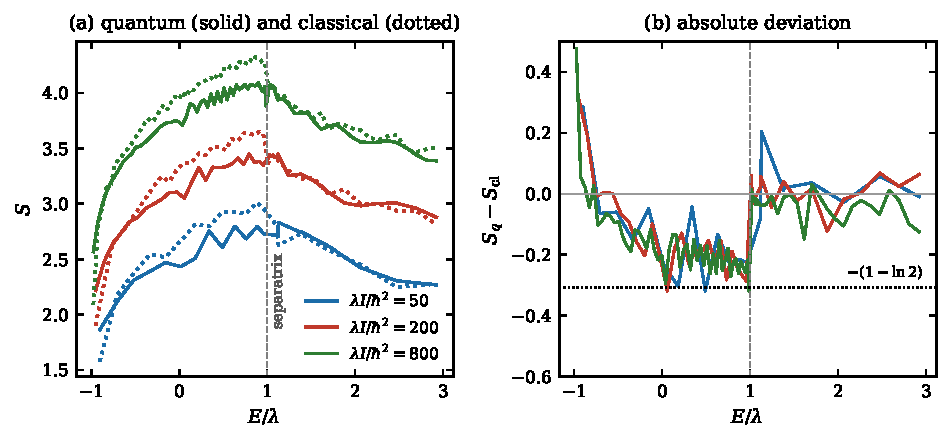
\includegraphics[width=\linewidth]{fig3_separatrix.pdf}
\caption{(a) Quantum entanglement entropy (solid) and classical coarse-grained
entropy (dotted) as functions of $\Erel/\lambda$ for $\lambda I/\hbar^{2}=50$,
$200$ and $800$. The dashed line marks the separatrix. (b) Absolute deviation
$S_{q}-\Scl^{\rm bin}$, with the asymptotic value $-(1-\ln2)$ of
\eqref{eq:main} shown dotted.}
\label{fig:separatrix}
\end{figure}

\emph{Agreement and deficit.} The curves track each other over the whole range.
The quantum entropy lies below the classical one throughout libration, by about
$0.2$, except within a few levels of the bottom of the well, where the band
covers only a handful of cells and the classical description fails; above the
separatrix it lies below by a smaller amount that grows with $\lambda$.
Relative to $S\approx3$--$4$ this is a few percent. Figure~\ref{fig:fringes}(a)
shows the mechanism: at $\lambda I/\hbar^{2}=800$, $\Erel/\lambda=1.54$ the
quantum weights oscillate about the classical envelope, the total-variation
distance between the two distributions is $0.33$, yet the entropies differ by
less than $1\%$. Figure~\ref{fig:fringes}(b) shows the deficit averaged over
energy windows as $\lambda$ grows from $200$ to $51\,200$: in libration it rises
from $0.18$ to $0.24$, in rotation from $0.01$ to $0.15$. Both increase
monotonically towards $1-\ln2$, but more slowly than in the pure Wannier--Stark
case, because at these couplings the bands contain only $10$--$500$ cells and
the caustic regions carry a large share of the weight.

\begin{figure}[t]
\centering
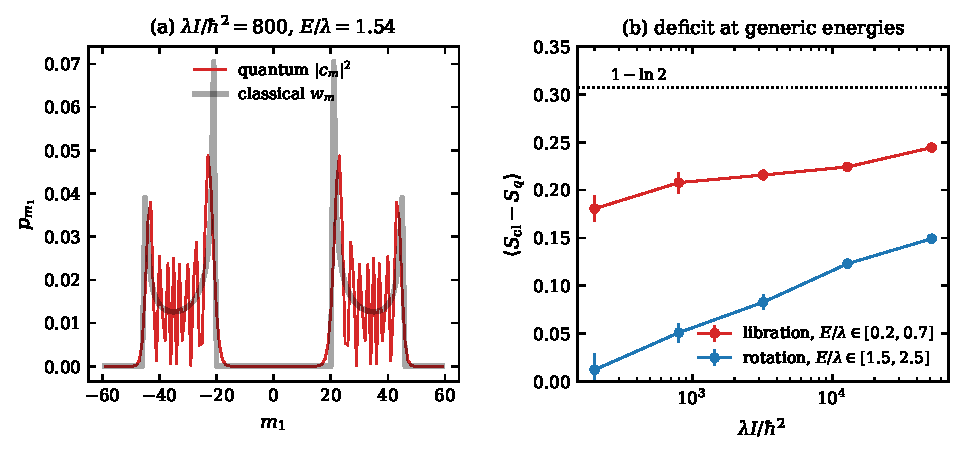
\includegraphics[width=\linewidth]{fig4_fringes.pdf}
\caption{(a) Momentum distribution of rotor 1 at $\lambda I/\hbar^{2}=800$,
$\Erel/\lambda=1.54$: the quantum weights (red) oscillate with full contrast
about the classical cell weights (grey), as \eqref{eq:fringesgen} predicts.
(b) Deficit $\langle\Scl^{\rm bin}-S_{q}\rangle$ averaged over energy windows in
libration and in rotation, against $\lambda$; error bars are standard errors
over the window.}
\label{fig:fringes}
\end{figure}

\emph{The separatrix.} Both entropies are maximal near $\Erel=\lambda$; for
$\lambda I/\hbar^{2}=50$, $200$ and $800$ the quantum maximum is at
$\Erel/\lambda=1.13$, $1.12$ and $0.90$. The classical reason is the cusp in the
support \eqref{eq:support}: the band of accessible momenta is widest at the
separatrix. On the quantum side this is where the non-degenerate librational
levels give way to the rotational doublets. The deviation in
Fig.~\ref{fig:separatrix}(b) changes abruptly there, because the fringe
structure changes: below the separatrix the two interfering branches are the two
halves of one libration orbit, above it the two halves of one rotation orbit,
and the band edges (caustics) move from $p=\pm\sqrt{I(\Erel+\lambda)}$ alone to
include $p=\pm\sqrt{I(\Erel-\lambda)}$. The separatrix of a classical system is
the locus of an excited-state quantum phase transition~\cite{CaprioCejnarIachello,
Stransky,Cejnar}, and the entropy maximum should be understood in that context.

%=============================================================================
\section{Deep libration}
\label{sec:libration}
%=============================================================================

\subsection{Harmonic approximation}

For $\lambda I/\hbar^{2}\gg1$ the ground state of $h$ is localised near the
minimum $\varphi=\pi$. Writing $x=\varphi-\pi$ and expanding
$\lambda\cos\varphi=-\lambda\cos x=-\lambda+\tfrac12\lambda x^{2}
-\tfrac{1}{24}\lambda x^{4}+O(x^{6})$,
\begin{equation}
h=-\lambda+\frac{p^{2}}{2\mu}+\frac12\mu\omega^{2}x^{2}-gx^{4}+\dots,\qquad
\mu=\frac{I}{2},\quad \mu\omega^{2}=\lambda,\quad g=\frac{\lambda}{24},
\label{eq:hho}
\end{equation}
so $\omega=\sqrt{2\lambda/I}$. Neglecting $g$, the ground state is
$u_{0}(x)\propto\exp(-\mu\omega x^{2}/2\hbar)$, with
$\langle x^{2}\rangle=\hbar/2\mu\omega$ and $\langle p^{2}\rangle=\mu\hbar\omega/2$.
Its Fourier coefficients are, up to the phase $e^{-ik\pi}$, a Gaussian in
$k=p/\hbar$ with variance
\begin{equation}
\sigma_{0}^{2}=\frac{\langle p^{2}\rangle}{\hbar^{2}}=\frac{\mu\omega}{2\hbar}
=\frac{I}{4\hbar}\sqrt{\frac{2\lambda}{I}}=\frac14\sqrt{\frac{2\lambda I}{\hbar^{2}}} .
\end{equation}
The wrap-around of the Gaussian on the circle is negligible when
$\langle x^{2}\rangle^{1/2}\ll\pi$, which holds here.

\subsection{Entropy of a sampled Gaussian}

For $p_{k}=e^{-k^{2}/2\sigma^{2}}/Z$ on the integers, Poisson summation gives
\begin{equation}
Z=\sum_{k\in\mathbb{Z}}e^{-k^{2}/2\sigma^{2}}
=\sqrt{2\pi}\,\sigma\left[1+2\sum_{\ell\ge1}e^{-2\pi^{2}\sigma^{2}\ell^{2}}\right],
\qquad
\sum_{k}k^{2}p_{k}=\sigma^{2}\left[1+O\!\left(\sigma^{2}e^{-2\pi^{2}\sigma^{2}}\right)\right].
\end{equation}
Since $-\ln p_{k}=\ln Z+k^{2}/2\sigma^{2}$,
\begin{equation}
S=\ln Z+\frac{\langle k^{2}\rangle}{2\sigma^{2}}
=\frac12\ln\left(2\pi e\sigma^{2}\right)
+O\!\left(\sigma^{2}e^{-2\pi^{2}\sigma^{2}}\right).
\end{equation}
The discreteness correction is exponentially small (below $10^{-8}$ already for
$\sigma^{2}\simeq1$). With $\sigma=\sigma_{0}$,
\begin{equation}
S_{0}=\frac12\ln\left(2\pi e\cdot\frac14\sqrt{\frac{2\lambda I}{\hbar^{2}}}\right)
=\frac12\ln\frac{\pi e}{2}+\frac14\ln2+\frac14\ln\frac{\lambda I}{\hbar^{2}}
=\frac14\ln\frac{\lambda I}{\hbar^{2}}+\frac12\ln\frac{\pi e}{\sqrt2},
\end{equation}
where $\tfrac12\ln(\pi e/2)+\tfrac14\ln2=\tfrac12\ln(\pi e\sqrt2/2)$ was used.

\subsection{The leading anharmonic correction}

The quartic term in \eqref{eq:hho} narrows the momentum distribution. To first
order in $g$ we need $\langle p^{2}\rangle$. The virial theorem follows from
$\langle[h,xp]\rangle=0$ in an eigenstate: since
$[p^{2}/2\mu,x]p=-i\hbar p^{2}/\mu$ and $x[V(x),p]=i\hbar xV'(x)$, it gives
$2\langle T\rangle=\langle xV'\rangle$. With $V=V_{2}-V_{4}$,
$V_{2}=\tfrac12\mu\omega^{2}x^{2}$, $V_{4}=gx^{4}$, one has
$xV'=2V_{2}-4V_{4}$, so $\langle V_{2}\rangle=\langle T\rangle+2\langle V_{4}\rangle$.
Inserting this into $E=\langle T\rangle+\langle V_{2}\rangle-\langle V_{4}\rangle$
gives $\langle T\rangle=\tfrac12(E-\langle V_{4}\rangle)$. To first order,
$E=\tfrac12\hbar\omega-g\langle x^{4}\rangle_{0}$ and
$\langle V_{4}\rangle=g\langle x^{4}\rangle_{0}$, so
\begin{equation}
\langle T\rangle=\tfrac14\hbar\omega-g\langle x^{4}\rangle_{0},\qquad
\langle x^{4}\rangle_{0}=3\langle x^{2}\rangle_{0}^{2}=\frac{3\hbar^{2}}{4\mu^{2}\omega^{2}} .
\end{equation}
Therefore
\begin{equation}
\langle p^{2}\rangle=2\mu\langle T\rangle=\frac{\mu\hbar\omega}{2}
-\frac{3g\hbar^{2}}{2\mu\omega^{2}}=\frac{\mu\hbar\omega}{2}-\frac{\hbar^{2}}{16},
\qquad
\sigma^{2}=\sigma_{0}^{2}-\frac{1}{16},
\end{equation}
where $g/\mu\omega^{2}=1/24$ was used. The quartic term also makes the
distribution non-Gaussian, but this does not change the entropy at first order.
If $p=\phi_{\sigma}(1+\epsilon\eta)$ with $\phi_{\sigma}$ the Gaussian of the
exact variance, then $\eta$ is orthogonal (with weight $\phi_{\sigma}$) to $1$,
$k$ and $k^{2}$, and
\begin{equation}
-\sum p\ln p=-\sum\phi_{\sigma}\ln\phi_{\sigma}
-\epsilon\sum\phi_{\sigma}\eta\left(1+\ln\phi_{\sigma}\right)+O(\epsilon^{2})
=S[\phi_{\sigma}]+O(\epsilon^{2}),
\end{equation}
because $\ln\phi_{\sigma}$ is a quadratic polynomial in $k$. Hence
$S=\tfrac12\ln(2\pi e\sigma^{2})$ to first order, and expanding
$\tfrac12\ln(\sigma_{0}^{2}-\tfrac1{16})=\tfrac12\ln\sigma_{0}^{2}-1/32\sigma_{0}^{2}
+\dots$,
\begin{equation}
\boxed{\;
S_{0}=\frac14\ln\frac{\lambda I}{\hbar^{2}}+\frac12\ln\frac{\pi e}{\sqrt2}
-\frac{1}{8\sqrt{2\lambda I/\hbar^{2}}}+O\!\left(\frac{\hbar^{2}}{\lambda I}\right)\;}
\label{eq:S0}
\end{equation}
with $\tfrac12\ln(\pi e/\sqrt2)=0.89908$. Figure~\ref{fig:libration} compares
this with exact diagonalisation. For $\lambda I/\hbar^{2}=10$, $40$, $160$,
$640$, $2560$ and $10240$ the residual after the harmonic terms is $-0.03027$,
$-0.01451$, $-0.00712$, $-0.00353$, $-0.00176$ and $-0.00088$, and its ratio to
the predicted correction is $1.083$, $1.039$, $1.019$, $1.009$, $1.005$ and
$1.002$, converging to unity as $O(\lambda^{-1/2})$.

\begin{figure}[t]
\centering
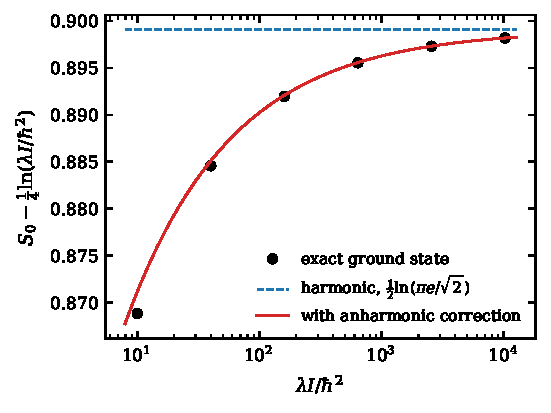
\includegraphics[width=0.55\linewidth]{fig5_libration.pdf}
\caption{Deep libration: $S_{0}-\tfrac14\ln(\lambda I/\hbar^{2})$ for the
ground state from exact diagonalisation (points), the harmonic constant
$\tfrac12\ln(\pi e/\sqrt2)$ (dashed), and \eqref{eq:S0} with the anharmonic
correction (solid).}
\label{fig:libration}
\end{figure}

%=============================================================================
\section{Discussion}
\label{sec:disc}
%=============================================================================

We have carried the programme of~\cite{DKS} from two coupled oscillators to two
coupled rotors. The central conclusion survives: in the semiclassical regime the
entanglement entropy of an eigenstate is reproduced, at the level of its leading
logarithm, by the Boltzmann entropy of the reduced classical phase-space
distribution, and this holds for a coupling that is not bilinear and across a
change in the topology of the classical orbits. The model is, however, rich
enough to show where and how the correspondence stops.

\emph{The cell is fixed, and the equality is not exact.} Compactness quantises
the angular momentum, so the classical distribution is coarse-grained onto the
integers that label the quantum Schmidt weights, and the comparison contains no
free constant. With nothing to adjust, the two entropies differ by
$1-\ln2$ in the semiclassical limit. We derived this in deep rotation, where the
quantum weights are exactly $J_{j}^{2}(\gamma)$ and the classical weights are the
arcsine law, and confirmed it numerically to $\gamma=10^{6}$; at generic
energies the same deficit is approached more slowly. In the language
of~\cite{DKS}, the classical formula reproduces the quantum entropy only if the
cell is taken as $eh/2$.

\emph{Why the oscillators and rotors differ.} The constant arises from the
interference of the two classical branches that correspond to one value of the
observed momentum. For the rotors, conservation of total angular momentum fixes
the Schmidt basis to be the angular-momentum basis, so the interference has
nowhere to go but into the Schmidt weights, where it appears as full-contrast
fringes. For the oscillators no conservation law fixes the Schmidt basis, the
reduced density matrix is doubly degenerate, and the interference is carried by
the eigenvectors. We expect the same distinction --- whether a symmetry ties the
Schmidt basis to the observable whose classical distribution is being compared
--- to decide the constant term in other systems.

\emph{Entropy and distribution are different statements.} At
$\lambda I/\hbar^{2}=800$ the quantum and classical momentum distributions have
total-variation distance $0.33$ while their entropies differ by less than one
percent. The classical--quantum correspondence for entanglement entropy is a
statement about one coarse functional of the state.

\emph{The separatrix.} Both entropies are maximal there, because the support of
the classical momentum distribution has a cusp maximum, and the deviation
between them changes abruptly as the fringe structure changes. The separatrix is
the classical locus of an excited-state quantum phase transition
(ESQPT)~\cite{CaprioCejnarIachello,Stransky,Cejnar}; entropic signatures of
ESQPTs have been studied, and the entropy maximum reported here should be
positioned with respect to that literature.

\emph{A point of technique.} The normalisation constant of a perturbed state is
of order $\lambda^{2}$ and may be dropped from a state kept to order $\lambda$.
It may not be dropped from the density matrix at the same order, because $\rho$
is bilinear in the amplitudes. Here it supplies the whole linear entropy and the
non-logarithmic part of the von Neumann entropy; omitting it gives a trace and a
purity larger than one and an entropy low by $10$--$14\%$. Checking
$\Tr\rho_{1}=1$ and $S_{L}\ge0$ at the order kept catches the omission.

\emph{Outlook.} Three extensions are natural. A quench of $\lambda$ across the
separatrix can be followed with the same Mathieu machinery and would show how
entanglement is generated dynamically. Coupling $N>2$ rotors makes the relative
motion non-integrable; whether the correspondence, and the constant $1-\ln2$,
survive chaos is the question most relevant to the high-energy setting that
motivated~\cite{DKS}. Finally, the Wannier--Stark structure of
Sec.~\ref{sec:rotation} suggests that the Bessel form of the Schmidt weights is
generic for any pair of systems with a conserved total charge and a linear
dispersion of the relative charge.

\begin{center}\rule{0.4\linewidth}{0.4pt}\end{center}

\appendix

%=============================================================================
\section{Integrals}
\label{app:integrals}
%=============================================================================

\paragraph{A.1. A logarithmic integral}
We show $\int_{0}^{\pi}\ln\sin u\,\dd u=-\pi\ln2$. Let
$I_{s}=\int_{0}^{\pi}\ln\sin u\,\dd u$. By symmetry about $\pi/2$,
$I_{s}=2\int_{0}^{\pi/2}\ln\sin u\,\dd u$, and by $u\to\pi/2-u$ also
$I_{s}=2\int_{0}^{\pi/2}\ln\cos u\,\dd u$. Adding,
\begin{equation}
2I_{s}=2\int_{0}^{\pi/2}\ln\left(\sin u\cos u\right)\dd u
=2\int_{0}^{\pi/2}\ln\frac{\sin2u}{2}\,\dd u
=\int_{0}^{\pi}\ln\sin v\,\dd v-\pi\ln2=I_{s}-\pi\ln2,
\end{equation}
with $v=2u$. Hence $I_{s}=-\pi\ln2$. Equivalently
$\int_{0}^{\pi}\ln|\cos t|\,\dd t=-\pi\ln2$.

\paragraph{A.2. Entropy of the arcsine law} For
$w(j)=1/(\pi\sqrt{\gamma^{2}-j^{2}})$ on $(-\gamma,\gamma)$ put
$j=\gamma\cos\beta$; then $w\,\dd j=\dd\beta/\pi$, uniform on $(0,\pi)$, and
$\gamma^{2}-j^{2}=\gamma^{2}\sin^{2}\beta$. Hence
\begin{equation}
-\int w\ln w\,\dd j=\ln\pi+\frac{1}{\pi}\int_{0}^{\pi}\ln\left(\gamma\sin\beta\right)
\dd\beta=\ln\pi+\ln\gamma-\ln2=\ln\frac{\pi\gamma}{2},
\end{equation}
using A.1.

\paragraph{A.3. The phase average} Split
$\frac{1}{2\pi}\int_{0}^{2\pi}(1+\cos\Phi)\ln(1+\cos\Phi)\,\dd\Phi=I_{1}+I_{2}$.
With $1+\cos\Phi=2\cos^{2}(\Phi/2)$ and A.1,
\begin{equation}
I_{1}=\frac{1}{2\pi}\int_{0}^{2\pi}\ln(1+\cos\Phi)\,\dd\Phi
=\ln2+\frac{2}{\pi}\int_{0}^{\pi}\ln|\cos t|\,\dd t=\ln2-2\ln2=-\ln2 .
\end{equation}
Integrating by parts with $\cos\Phi\,\dd\Phi=\dd\sin\Phi$ (the boundary term
vanishes, including at $\Phi=\pi$ where $\sin\Phi\ln(1+\cos\Phi)\to0$),
\begin{equation}
I_{2}=\frac{1}{2\pi}\int_{0}^{2\pi}\cos\Phi\ln(1+\cos\Phi)\,\dd\Phi
=\frac{1}{2\pi}\int_{0}^{2\pi}\frac{\sin^{2}\Phi}{1+\cos\Phi}\,\dd\Phi
=\frac{1}{2\pi}\int_{0}^{2\pi}(1-\cos\Phi)\,\dd\Phi=1 .
\end{equation}
The sum is $1-\ln2$.

\paragraph{A.4. The elliptic integral near the separatrix} For
$k\to1$, $\mathsf{K}(k)=\ln(4/k')+O(k'^{2}\ln k')$ with $k'=\sqrt{1-k^{2}}$, the
standard logarithmic singularity~\cite{AbramowitzStegun}; it is the divergence of
the classical period at the separatrix used in Sec.~\ref{sec:classical}.

%=============================================================================
\section{Numerical methods and verification}
\label{app:num}
%=============================================================================

All numerics use $\hbar=I=1$. Sector Hamiltonians \eqref{eq:hsector} are
diagonalised densely with truncation $|m_{i}|\le N$, convergence being checked
by varying $N$ and requiring the weight on boundary states to be below
$10^{-6}$. For the pendulum sectors we use $N=8\sqrt{\lambda}+150$ and
diagonalise separately in the two parity sectors (Sec.~\ref{sec:pendulum}).
Where exponentially degenerate exchange doublets are returned as mixtures, the
branch entropy is obtained from the weight on one side of $m_{1}=M/2$,
renormalised. Classical cell weights \eqref{eq:Sbin} are computed by adaptive
quadrature, with the band-edge singularities supplied to the routine; for the
arcsine law they are evaluated in closed form,
$w_{j}=\pi^{-1}[\arcsin(j_{+}/\gamma)-\arcsin(j_{-}/\gamma)]$ with $j_{\pm}$ the
cell edges clipped to $[-\gamma,\gamma]$. Bessel weights are summed over
$|j|\le\gamma+40\gamma^{1/3}+50$, where the neglected tail is below
$10^{-10}$. Table~\ref{tab:checks} collects the comparisons quoted in the text.

\begin{table}[h]
\centering
\caption{Analytic results of this paper against exact numerics
($\hbar=I=1$). Unless stated, perturbative checks are at $n=7$
($m_{1}=9$, $m_{2}=2$) and $\lambda=0.02$; Mathieu checks at $q=14.6$.}
\label{tab:checks}
\small
\renewcommand{\arraystretch}{1.15}
\begin{tabular}{lll}
\toprule
quantity & analytic & numerical\\
\midrule
$c_{+}$, Eq.~\eqref{eq:first} & -0.0012500 & -0.0012500 \\
$c_{-}$, Eq.~\eqref{eq:first} & 0.0016667 & 0.0016667 \\
$c_{++}$, Eq.~\eqref{eq:second} & $6.944444\times10^{-7}$ & $6.944456\times10^{-7}$ \\
$c_{--}$, Eq.~\eqref{eq:second} & $1.666667\times10^{-6}$ & $1.666669\times10^{-6}$ \\
$E^{(2)}$, Eq.~\eqref{eq:E2} & $4.166667\times10^{-6}$ & $4.166668\times10^{-6}$ \\
$p_{0}=1-\epsp-\epsm$ at $\lambda=0.4$ & 0.9982639 & 0.9982649 \\
$S$ at $n=0$, $\lambda=0.02$, Eq.~\eqref{eq:Sweak} & 0.0020420 & 0.0020411 \\
$S$ at $n=30$, $\lambda=0.05$, Eq.~\eqref{eq:Sasym} & $2.108355\times10^{-5}$ & $2.114621\times10^{-5}$ \\
$M=0$ lowest level vs $a_{0}(q)/4$ & -5.4542890 & -5.4542890 \\
$M=0$ third level vs $a_{2}(q)/4$ & 1.3368673 & 1.3368673 \\
$M=1$ lowest level vs $b_{1}(q)/4$ & -5.4542787 & -5.4542787 \\
$M=1$ second level vs $a_{1}(q)/4$ & -1.9036729 & -1.9036729 \\
$B$, $\Erel=300$, $\lambda=100$, Eqs.~\eqref{eq:Brot},\eqref{eq:Blib} & 0.0927037 & 0.0927037 \\
$B$, $\Erel=60$, $\lambda=100$, Eqs.~\eqref{eq:Brot},\eqref{eq:Blib} & 0.1596085 & 0.1596085 \\
$p_{j=0}$ at $n=400$, $\gamma=5$ vs $J_{0}^{2}(5)$ & 0.0315406 & 0.0314917 \\
$p_{j=3}$ at $n=400$, $\gamma=5$ vs $J_{3}^{2}(5)$ & 0.1331018 & 0.1343519 \\
arcsine entropy $\ln(\pi\gamma/2)$, $\gamma=10^{4}$ & 9.6619231 & 9.6619231 \\
$\Scl^{\rm bin}-S_{q}$ at $\gamma=10^{6}$ vs $1-\ln2$ & 0.3068528 & 0.2978385 \\
$S_{0}$ at $\lambda I/\hbar^{2}=10240$, Eq.~\eqref{eq:S0} & 3.2067189 & 3.2067169 \\
$N_{\rm lib}$ at $\lambda I/\hbar^{2}=800$ vs $(4/\pi)\sqrt q$ & 50.92958 & 51.00000 \\
\bottomrule
\end{tabular}
\end{table}

\noindent The scripts that produce every figure and table are available from
the authors.

\begin{thebibliography}{99}

\bibitem{AmicoRMP} L.~Amico, R.~Fazio, A.~Osterloh, V.~Vedral,
Rev.\ Mod.\ Phys.\ \textbf{80} (2008) 517.
\bibitem{HorodeckiRMP} R.~Horodecki, P.~Horodecki, M.~Horodecki, K.~Horodecki,
Rev.\ Mod.\ Phys.\ \textbf{81} (2009) 865.
\bibitem{EisertRMP} J.~Eisert, M.~Cramer, M.~B.~Plenio,
Rev.\ Mod.\ Phys.\ \textbf{82} (2010) 277.
\bibitem{KharzeevLevin} D.~E.~Kharzeev, E.~M.~Levin,
Phys.\ Rev.\ D \textbf{95} (2017) 114008.
\bibitem{Kutak} K.~Kutak, Phys.\ Lett.\ B \textbf{705} (2011) 217.
\bibitem{Hagiwara} Y.~Hagiwara, Y.~Hatta, B.-W.~Xiao, F.~Yuan,
Phys.\ Rev.\ D \textbf{97} (2018) 094029.
\bibitem{DKS} H.~Duan, A.~Kovner, V.~V.~Skokov,
\emph{Classical entanglement and entropy}, arXiv:2301.05735 [quant-ph] (2023).
\bibitem{CaprioCejnarIachello} M.~A.~Caprio, P.~Cejnar, F.~Iachello,
Ann.\ Phys.\ \textbf{323} (2008) 1106.
\bibitem{Stransky} P.~Str\'ansk\'y, M.~Macek, P.~Cejnar,
Ann.\ Phys.\ \textbf{345} (2014) 73.
\bibitem{Cejnar} P.~Cejnar, P.~Str\'ansk\'y, M.~Macek, M.~Kloc,
J.~Phys.\ A \textbf{54} (2021) 133001.
\bibitem{DLMF28} NIST Digital Library of Mathematical Functions, Chapter~28
(Mathieu functions), \url{https://dlmf.nist.gov/28}.
\bibitem{DLMF10} NIST Digital Library of Mathematical Functions, \S10.19
(asymptotic expansions of Bessel functions for large order),
\url{https://dlmf.nist.gov/10.19}.
\bibitem{AbramowitzStegun} M.~Abramowitz, I.~A.~Stegun, \emph{Handbook of
Mathematical Functions}, Dover, New York, 1972, Chs.~17 and 20.

\end{thebibliography}

\end{document}
